\chapter{Wind Turbine Control}  \label{sec:Application to Wind Turbine Control4}

%Modern megawatt wind turbines are both speed-controlled and pitch-controlled \cite{pao2011control, mulders2018delft, elkodama2023control}. Controllers and their parameters are often fine-tuned to fit not only a specific wind turbine type but also individual turbines, taking into account factors such as manufacturing and installation variations, including rotor blade weight imbalances and aging processes \cite{en14238083}. These conventional feedback control designs, typically relying solely on generator speed as input and controlling the blade pitch angles collectively, are well-engineered and technologically mature. However, further reduction of the cost of energy production can be achieved by introducing additional control inputs or sensors. Moreover, using a predictive scheme like qLMPC allows leveraging wind measurements or estimates and incorporating this information over a prediction horizon. It also accounts for how the system states, e.g., the rotor and generator speed, are expected to react to the wind trajectory and future control inputs within that horizon. This chapter investigates control strategies that leverage such improvements: a qLMPC design, which incorporates preview wind information, and PI Individual Pitch Control (IPC), the latter both as a standalone method and in combination with Trailing Edge Flap Control (TEFC), aimed at reducing mechanical loads. These control approaches are evaluated in terms of power reference tracking, actuator activity, and mechanical loads.
%In Section~\ref{sec:quasiLPVMPCDesign}, the design of a velocity-based qLMPC controller based on a first-principles model is presented. Section~\ref{section:Individal Pitch PI Control} introduces IPC, explaining the multi-blade coordinate transformation and comparing IPC simulation results to those from baseline Collective Pitch Control (CPC). Section~\ref{sec:CombinedIPC-TrailingEdgeFlapControl} describes the combination of IPC and TEFC, including the necessary model extensions and the achieved load reductions on the blades and tower. A brief comparison and conclusion section summarizes the results obtained with the three wind turbine controller designs. The results for the qLMPC controller have been published in \cite{dittmer2021velocity}, and the TEFC control strategy in \cite{dittmer2024combined}.
%  
Modern megawatt wind turbines are both speed-controlled and pitch-controlled \cite{pao2011control,
    mulders2018delft, elkodama2023control}. Controllers and their parameters are often fine-tuned to
fit not only a specific wind turbine type but also individual turbines, taking into account factors
such as manufacturing and installation variations, including rotor blade weight imbalances and
aging processes \cite{en14238083}. These conventional feedback control designs, typically relying
solely on generator speed as input and controlling the blade pitch angles collectively, are
well-engineered and technologically mature. However, further reduction of the cost of energy
production can be achieved by introducing additional control inputs or sensors. Moreover, using a
predictive scheme like qLMPC allows leveraging wind measurements or estimates and incorporating
this information over a prediction horizon. It also accounts for how the system states, e.g., the
rotor and generator speed, are expected to react to the wind trajectory and future control inputs
within that horizon. This chapter investigates control strategies that leverage such improvements:
a qLMPC design, which incorporates preview wind information, and PI Individual Pitch Control
(IPC), the latter both as a standalone method and in combination with Trailing Edge Flap Control
(TEFC), aimed at reducing mechanical loads. These control approaches are evaluated in terms of
power reference tracking, actuator activity, and mechanical loads.

In Section~\ref{sec:quasiLPVMPCDesign}, the design of a velocity-based qLMPC controller based on
the first-principles model of Chapter~\ref{sec:WindTurbineqLPVModels} is presented. Where qLMPC
has so far been applied to wind turbines as a SISO scheme \cite{mulders2020preventing, pamososuryo2022individual,
    fonseca2024windTurbineSideSide}, the design presented here actuates generator torque and
collective pitch simultaneously as a MIMO scheme, covering the entire operating range. It is
reformulated as a QP and solved via a linear complementarity formulation with Lemke's algorithm
\cite{cisneros2020velocity}, yielding mean solver times below 2\,ms at a controller sampling time
of 8\,ms and thus real-time capability.
%
Section~\ref{section:Individal Pitch PI Control} introduces IPC, explaining the multi-blade
coordinate transformation and comparing IPC simulation results to those from baseline Collective
Pitch Control (CPC). The simulation environment is also used to tune the IPC gains, by a grid
search followed by a Nelder-Mead simplex optimization of the blade root DEL.
%
Section~\ref{sec:CombinedIPC-TrailingEdgeFlapControl} describes the combination of IPC and TEFC,
including the necessary model extensions and the achieved load reductions on the blades and tower.
Whereas earlier studies combining the two actuation principles report results for single mean wind
speeds \cite{wilson2009combined, henriksen2013model, he2018combined}, the controller presented
here is demonstrated across Regions II and III, using one training data set and two independent
verification data sets. A final comparison section evaluates qLMPC, IPC, and AALC against each
other, showing the trade-off between DEL reduction and actuator activity relative to the PI CPC
baseline. The results for the qLMPC controller have been published in \cite{dittmer2021velocity},
and the TEFC control strategy in \cite{dittmer2024combined}.
\section{qLMPC Design and Application}\label{sec:quasiLPVMPCDesign}
Wind turbine controller design in above rated region focuses on smooth power control and in the below rated region on power optimization, as described in \cite{Bianchi2007}. Generator speed reference tracking is achieved using two control inputs: the collective blade pitch angle $\beta_{0,\text{ref}}$ and the generator torque reference $T_{g,\text{ref}}$. The baseline controller consists of two SISO controllers, one for generator torque and one for blade pitch control, see Section~\ref{sec:WindTurbineControl}. These can be replaced by a MIMO qLMPC power controller, see Figure \ref{fig:BlockMPC}. The qLMPC is designed to track rotor and generator speed references while minimizing changes in the control inputs, resulting in smoother power output and reduced tower movement compared to the baseline. DEL reduction is not an explicit objective of the qLMPC design. However, the five evaluation criteria used to compare all control strategies introduced in Section~\ref{subsection Control Objectives}, i.e., blade and tower DEL, power mean and variance, and actuator activity, are also calculated for this controller to enable a direct comparison with the IPC and AALC designs.

\begin{figure}[ht]
    \centering
    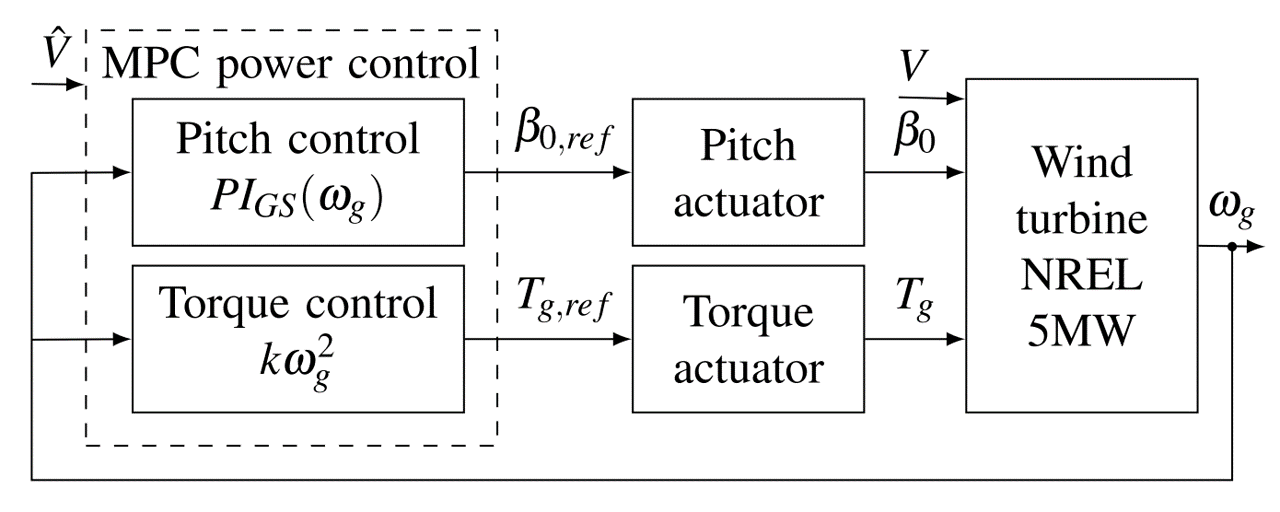
\includegraphics[width=0.8\textwidth,trim={0 0cm 0cm 0.3cm},clip]{figures/Figures_ADi/turbineMPC.png}
    \caption[Block diagram of the closed-loop wind turbine control structure with qLMPC replacing the baseline PI controller]{Block diagram of the closed-loop wind turbine control structure with qLMPC (dashed box) replacing the baseline PI controller (solid line)}
    \label{fig:BlockMPC}
\end{figure}

In this work, the velocity based approach from \cite{cisneros2020velocity}, presented in section \ref{windTurbineModel} of this thesis, is applied: A $3^{rd}$ order wind turbine model, used as the basis for quasiLPV based MIMO controller design in \cite{Bianchi2007}, is implemented with some minor changes. To model the main dynamics, it is sufficient to consider the slip angle $\theta_s$, the rotor and generator speed $\omega_r$ and $\omega_g$. The same states are considered here, but three modifications were made:
\begin{enumerate}
    \item A filtered generator torque $T_g^{\prime} = T_{g,\text{ref}}$ is introduced as an additional state to eliminate direct throughput, i.e., to avoid a non-zero feedthrough matrix \( \bm{D} \). This fourth state enables the use of the optimization framework for reference tracking and disturbance rejection proposed in \cite{cisneros2020velocity}. Incorporating a filtered control input as an additional state is a common practice, and is, for example, also employed in the MPC algorithm implemented in WFSim \cite{boersma2018control}.    
    \item Reference generator torque $T_{g,\text{ref}}$ is used as a control output signal and plant input signal. In \cite{Bianchi2007}, the second control input is the zero torque speed $\omega_Z$ which is linearly dependent on the generator torque $T_{g}$. The reference torque is selected as it is the format of expected input signal to the wind turbine in the FAST implementation. The optimal trajectory of the reference generator torque  $T_{g,\text{ref}}$ over a prediction horizon is calculated based on an optimal reference signal $r_{\beta}$ which is itself calculated from the wind speed.
    \item A desired pitch signal $r_{\beta}$ is used as a reference for the prediction horizon in the MPC optimization to calculate the optimal controller output pitch signal $\beta_{0,\text{ref}}$. In \cite{Bianchi2007}, a reference value for the generator speed is tracked. This choice was made to directly optimize the two actuators to avoid handling the large difference in dynamic bandwidth of the actuators and the plant dynamics in the optimization calculation. Identical to the filtered generator torque, a filtered pitch $\beta_0^{\prime} = \beta_{0,\text{ref}}$ is introduced as a fifth state.
\end{enumerate}
%
The resulting states, input and output vectors are given below. As before, different indices are used for the generator speed in the high-speed shaft, denoted $\omega_g$, and the low-speed shaft, $\omega_{gr}$. In the state vector, the generator speed in the low-speed shaft is used as it operates in the same reference system as the rotor speed $\omega_r$:
\begin{align}\label{eq:xMPCyMPC}
    \bm{x}_{\text{MPC}} =[\theta_{s}  \quad {\omega}_r \quad {\omega}_{gr} \quad T_g^{\prime} \quad \beta_0^{\prime} ]^T  \in \mathbb{R}^{5 \times 1},   \quad \bm{y}_{\text{MPC}} = [T_{g,\text{ref}} \quad  {\beta}_{0,\text{ref}}]^T  \in \mathbb{R}^{2 \times 1}.
\end{align}
%
The nonlinear dynamics describing changes in the three turbine states are:
\begin{align}
    \dot{\theta_s}(t)&={\omega}_r(t)-{\omega}_{gr}(t) \label{eq:NLDyn1}\\
    \dot{\omega}_r(t)&=-\frac{K_{sr}}{J_r}\theta_s(t)-\frac{B_{sr}}{J_r}{\omega}_r(t)+\frac{B_{sr}}{J_r}{\omega}_{gr}(t)+\frac{T_r({\omega}_r, \beta, v)}{J_r}\\
    \dot{\omega}_{gr}(t)&=\frac{K_{sr}}{J_{gr}}\theta_s(t)+\frac{B_{sr}}{J_{gr}}{\omega}_r(t)-\frac{B_{sr}}{J_{gr}}{\omega}_{gr}(t)-\frac{N_gT_g(t)}{J_{gr}} \label{eq:NLDyn3} \\
 %   \dot{ T}^{\prime}_{g} &= -\frac{1}{ \kappa}T_{g} +\frac{1}{ \kappa}T_{g, ref}\\
%    \dot{\beta}^{\prime}_& = -\frac{1}{ \tau}\beta^{\prime} +\frac{1}{ \tau}\beta_{g, ref}
\end{align}
%
To avoid having to derive a grid of initial states for the different combinations of the state vector, a velocity based linearization is designed.
\subsection{Velocity-Based qLPV Model Linearization}
The velocity-based linearization method from \cite{cisneros2020velocity} is implemented for the model serving as the basis of the qLMPC design. The nonlinear system dynamics
\[
\dot{\bm{x}}_{\text{MPC}}(t) = \bm{f}_{\text{MPC}}(\bm{x}_{\text{MPC}}, \bm{w}_{\text{Mdl}}), \quad \bm{y}_{\text{MPC}}(t) = \bm{h}_{\text{MPC}}(\bm{x}_{\text{MPC}})
\]
are described by the relationship between the state and input derivatives: 
\begin{align*}
    \ddot{\bm{x}}_{\text{MPC}}(t) &= \nabla_{\bm{x}_{\text{MPC}}} \bm{f}_{\text{MPC}}(\bm{x}_{\text{MPC}}, \bm{w}_{\text{Mdl}}) \dot{\bm{x}}_{\text{MPC}}(t) + \nabla_{\bm{w}_{\text{Mdl}}}\bm{f}_{\text{MPC}}(\bm{x}_{\text{MPC}}, \bm{w}_{\text{Mdl}}) \dot{\bm{w}}_{\text{Mdl}}(t),\\
    \dot{\bm{y}}_{\text{MPC}}(t) &= \nabla_{\bm{x}_{\text{MPC}}}\bm{h}_{\text{MPC}}(\bm{x}_{\text{MPC}}) \dot{\bm{x}}_{\text{MPC}}(t).   
\end{align*}
By considering the derivatives instead of the original states, the need for storing steady-state vectors for input, output, and states at each operating point is omitted.
%

The continuous-time system, input, and output matrices,
\begin{align*}
      \bm{A}_c(\bm{\rho}_{\Rho}) &= \nabla_{\bm{x}_{\text{MPC}}} \bm{f}(\bm{x}_{\text{MPC}}, \bm{w}_{\text{Mdl}}),\\ 
      \bm{B}_c(\bm{\rho}_{\Rho}) &= \nabla_{\bm{w}_{\text{Mdl}}} \bm{f}(\bm{x}_{\text{MPC}}, \bm{w}_{\text{Mdl}}),\\ 
      \bm{C}_c(\bm{\rho}_{\Rho}) &= \nabla_{\bm{x}_{\text{MPC}}} \bm{h}(\bm{x}_{\text{MPC}}),
\end{align*}
where the scheduling parameter $\bm{\rho}_{\Rho}$ consists of the measurement values of  wind speed $V_{\infty}$, pitch angle $\beta_0$ and rotor speed $\omega_r$,
\[\rho_{P} = [V_{\infty} \quad {\beta_0} \quad {\omega}_{r} ]\in \mathbb{R}^{1 \times 3}, \]  
with the corresponding state vector $\bm{x}_{\text{MPC}}$ and output vector $\bm{y}_{\text{MPC}}$ as defined in Equation~\ref{eq:xMPCyMPC} and $w_{\text{Mdl}} = [V_{\infty} \; \; T_g  \; \; \beta_0]$. Although the control scheme is velocity-based, i.e., based on state derivatives or, in discrete time, state differences, the scheduling parameters are taken in their original non-derivative form. This is because the partial derivatives such as \( \partial T_r / \partial \omega_r \), \( \partial T_r / \partial \beta \), and \( \partial T_r / \partial V_{\infty} \), are functions of the current physical states, not their time derivatives.

The matrices depend on the physical parameters described in Section \ref{sec:MechanicalAerodynamicSubsystemModel} and can be set up from Equations~\eqref{eq:NLDyn1} to~\eqref{eq:NLDyn3}:  
\begin{equation}
    \begin{aligned}
        \bm{A}_c(\bm{\rho}_{\Rho}) &=
        \begin{bmatrix}
            0  & 1 & -1 & 0 & 0 \\ 
            -\frac{K_{sr}}{J_r}  & -\frac{B_{sr}}{J_r} + \frac{1}{J_r}\frac{\partial T_r}{\partial{\omega_r}} & \frac{B_{sr}}{J_r} & 0 & \frac{1}{J_r}\frac{\partial T_r}{\partial{\beta}} \\ 
            \frac{K_{sr}}{J_{gr}} & \frac{B_{sr}}{J_{gr}} & -\frac{B_{sr}}{J_{gr}} & -\frac{N_g}{J_{gr}} & 0 \\ 
            0 & 0 & 0 & -\frac{1}{\kappa} & 0 \\ 
            0 & 0 & 0 & 0 & -\frac{1}{\tau} 
        \end{bmatrix} \in \mathbb{R}^{5 \times 5},\\
\bm{B}_c(\bm{\rho}_{\Rho}) &=
\left[
\begin{array}{c|cc}
    0 & 0 & 0 \\
    \frac{1}{J_r}\frac{\partial T_r}{\partial V_{\infty}} & 0 & 0 \\
    0 & 0 & 0 \\
    0 & \frac{1}{\kappa} & 0 \\
    0 & 0 & \frac{1}{\tau}
\end{array}
\right]
=
\begin{bmatrix}
    \bm{B}_{c,V} & \bm{B}_{c,u}
\end{bmatrix}
\in \mathbb{R}^{5 \times 3}\\
        \bm{C}_c &=
        \begin{bmatrix}
            0 & 0 & 0 & 1 & 0 \\
            0 & 0 & 0 & 0 & 1
        \end{bmatrix} \in \mathbb{R}^{2 \times 5}.
    \end{aligned}
\end{equation}
%
The wind affects the system through the first column of the input matrix, denoted here as $\bm{B}_{c,V}$. The wind speed $V_{\infty}$ cannot be controlled and only its current value is assumed to be known and constant over the prediction horizon. Nevertheless, the column $\bm{B}_{c,V}$ must be retained, as the change in wind speed $\Delta V_{\infty}$ is treated as a disturbance input between time steps. To reflect this structure, the input matrix $\bm{B}_c$ is partitioned into the wind disturbance input $\bm{B}_{c,V}$ in the first column and the control input influence $\bm{B}_{c,u}$ in the second and third columns. For implementation in the predictive controller, the wind-dependent column is moved into the system matrix as an additional state, since it represents a known but uncontrollable input.

This continuous LPV model needs to be discretized for its application in a real-time qLMPC design. The model in discretized form is:
\begin{align}\label{eq4:DiscreteForm}
    \Delta \bm{x}_{\text{MPC},k}(k+1) = \bm{A}_{k}(\bm{\rho}_\Rho)\Delta \bm{x}_{\text{MPC},k}(k) + \bm{B}_{k}(\bm{\rho}_\Rho) \Delta \bm{w}_{\text{Mdl},k}(k)
\end{align}
with the discretized system and input matrices $\bm{A}_k \in \mathbb{R}^{5 \times 5}$ and $\bm{B}_k  \in \mathbb{R}^{5 \times 3}$ dependent on scheduling parameter vector $\bm{\rho}_{P}$ at the $k^{\text{th}}$ sample.
%
%
As in \cite{cisneros2019wide} the 4$^{th}$ order discretized state space representation to derive the matrices  $\bm{A}_k$ and $\bm{B}_k$ is implemented as:
\begin{align*}
    \bm{A}_{k}(\bm{\rho}_\Rho) &= \frac{T_s^4}{24}\bm{A}_c^4(\bm{\rho}_\Rho) + \frac{T_s^3}{6}\bm{A}_c^3(\bm{\rho}_\Rho) + \frac{T_s^2}{2}\bm{A}_c^2(\bm{\rho}_\Rho) + T_s \bm{A}_c(\bm{\rho}_\Rho)+ I,\\
    \bm{B}_{k}(\bm{\rho}_\Rho) &= \frac{T_s^3}{24}\bm{A}_c^3(\bm{\rho}_\Rho)\bm{B}_c(\bm{\rho}_\Rho) + \frac{T_s^2}{6}\bm{A}_c^2(\bm{\rho}_\Rho) \bm{B}_c(\bm{\rho}_\Rho) + \frac{T_s}{2} \bm{A}_c(\bm{\rho}_\Rho) \bm{B}_c(\bm{\rho}_\Rho)
    + \bm{B}_c(\bm{\rho}_\Rho).
\end{align*}
%
The discrete-time outputs can be calculated as the sum of the former sampled outputs and their current change:
\begin{align*}
    T_g^{\prime} (k+1)= T^{\prime}_g(k)  + \Delta T^{\prime} _g(k+1), \quad \beta^{\prime}_0(k+1) = \beta^{\prime}_0(k) + \text{Act}^{\prime}_0 (k+1).
\end{align*}
With this, the discrete state at step $k+1$ is calculated as:
\[
\begin{bmatrix}
    \bm{y}_{\text{MPC},k+1}  \\
    \Delta \bm{x}_{\text{MPC},k+1}
\end{bmatrix} = \begin{bmatrix}
    \bm{I}_{2\times2} &  \bm{A}_{k,y}(\bm{\rho}_P)  \\
    \bm{0}_{5\times2} & \bm{A}_{k}(\bm{\rho}_P)
\end{bmatrix} \begin{bmatrix}
    \bm{y}_{\text{MPC},k} \\
    \Delta \bm{x}_{\text{MPC},k}
\end{bmatrix} + \begin{bmatrix}
    \bm{B}_{k,y}(\bm{\rho}_P)    \\
    \bm{B}_{k}(\bm{\rho}_P)
\end{bmatrix} \Delta \bm{w}_{\text{Mdl},k}
\]
with $\bm{A}_{k,y} \in \mathbb{R}^{5 \times 2}$ and $\bm{B}_{k,y} \in \mathbb{R}^{2 \times 2}$ denoting the rows of the matrices corresponding to the outputs. The new state vector $\bm{x}_{\text{MPC}^\prime} = [y_{\text{MPC}}^T \quad \Delta  \bm{x}_{\text{MPC}}^T]^T$ is then
\begin{align} \label{eq:stateMPC}
    \bm{x}_{\text{MPC}^\prime} = \begin{bmatrix}T_g^{\prime} & \beta_0^{\prime} & \Delta \theta_s  & \Delta \omega_r & \Delta \omega_{g,r} & \Delta T_g & \text{Act}_0 \end{bmatrix}^T \in \mathbb{R}^{7 \times 1}.
\end{align}
%
\subsection{qLMPC Model for Reference Tracking}
Generally, the steady-state vector $\bm{x}_{s} \in \mathbb{R}^{n_x \times 1}$ and the corresponding steady-state control input $\bm{u}_{s} \in \mathbb{R}^{n_u \times 1}$ are determined based on the equilibrium of the system, which is defined as:
\begin{align*}
    \bm{x}_{s}(t + T_s) = \bm{x}_{s}(t),  \quad \bm{u}_{s}(t + T_s) = \bm{u}_{s}(t), \quad
    \bm{e}_s(t) = \bm{r} - \bm{C} \bm{x}_{s}(t) = \bm{0}_{n_y \times 1}, 
\end{align*}
%
where $\bm{e}_s(t) \in \mathbb{R}^{n_y \times 1}$ is the steady-state error, $\bm{r} \in \mathbb{R}^{n_y \times 1}$ is the reference signal, $\bm{C} \in \mathbb{R}^{n_y \times n_x}$ is the output matrix, and $T_s$ is the sampling time. This leads to the steady-state solution:
\begin{align} \label{eq:steadystatevec}
    \bm{x}_{\text{MPC}^\prime,s} =  \begin{bmatrix} r_{T_g} & r_{\beta} & 0 & 0 & 0 & 0 & 0 \end{bmatrix}^T, \quad
    \Delta{\bm{u}}_{\text{Mdl},s} = \begin{bmatrix} 0 & 0 \end{bmatrix}^T.
\end{align}
where \(r_{T_g}\) and \(r_{\beta}\) denote the reference generator torque and pitch, respectively, and $\Delta{\bm{u}}_{\text{Mdl},s} \in \mathbb{R}^{2 \times 1}$ is the deviation of the corresponding steady-state control input $\bm{u}_{\text{Mdl},s}$. This deviation should be zero in steady state. All elements of the vector in Equation~\eqref{eq:steadystatevec} that represent state deviations are therefore set to zero, i.e., the third to seventh elements, corresponding to the state vector in Equation~\eqref{eq:stateMPC}.  
The notable exceptions are the first two elements, which do not represent derivatives but rather the outputs \( T_g \) and \( \beta_0 \). These should converge to their respective steady-state values \( r_{T_g} \) and \( r_{\beta} \), which are determined based on the current wind speed and the look-up tables for thrust and torque coefficients.

The control input vector is defined as the two control inputs contained in $w_{\text{Mdl}} = [V_{\infty} \quad T_g \quad \beta_0]$ as
\begin{align*}
    \bm{u}_{\text{Mdl}} = \begin{bmatrix} T_g & \beta_0 \end{bmatrix},
\end{align*} 
and the control input for the discrete velocity based form is %as provided in Equation \ref{eq4:DiscreteForm}
\begin{align} \label{eq:DeltaUinput}
    \Delta \bm{u}_{\text{Mdl}} = \begin{bmatrix} \Delta T_g & \text{Act}_0  \end{bmatrix}. 
\end{align} 
% \[x=[\theta_{s}  \quad {\omega}_r \quad {\omega}_{gr} \quad T_g  ]^T \]
%\[u=\begin{bmatrix} V  & \beta_{ref} & T_{g,ref}  \end{bmatrix}\]
%
For MPC the augmented discrete time state space model can be written as:
\begin{align*}
    \begin{bmatrix}
        \bm{y}_{\text{MPC}}(k+1)  \\
        \Delta \bm{x}_{\text{MPC}}(k+1)
    \end{bmatrix} = \begin{bmatrix}
        \bm{I}_{2} & \bm{A}_{k,y}(\bm{\rho}_P)  \\
        \bm{0}_{5\times2} & \bm{A}_k(\bm{\rho}_P)
    \end{bmatrix}
    \begin{bmatrix}
        \bm{y}_{\text{MPC}}(k) \\
        \Delta \bm{x}_{\text{MPC}}(k)
    \end{bmatrix} 
    + 
    \begin{bmatrix}
        \bm{B}_{k,y,v}(\bm{\rho}_P)  \\  
        \bm{B}_{k,v}(\bm{\rho}_P) 
    \end{bmatrix}\Delta V_{\infty}(k) 
    \\+
    \begin{bmatrix}
        \bm{B}_{k,y,u}(\bm{\rho}_P)     \\
        \bm{B}_{k,u}(\bm{\rho}_P) 
    \end{bmatrix}\Delta \bm{u}_{\text{Mdl}}(k)
\end{align*}
where $\bm{B}_{k,v} \in \mathbb{R}^{5 \times 1}$ and $\bm{B}_{k,u} \in \mathbb{R}^{5 \times 2}$ are the columns of the input matrix related to the changes in the disturbance input, i.e., wind speed $\Delta V_{\infty}$, and the two control inputs, respectively, acting on the changes in states. The matrices $\bm{B}_{k,y,v} \in \mathbb{R}^{2 \times 1}$ and $\bm{B}_{k,y,u} \in \mathbb{R}^{2 \times 2}$ influence directly the two control signals in the vector $ \bm{y}_{\text{MPC}}$. The wind is considered to only change at the first sample of the prediction horizon. This reflects that the wind measurement or estimate at each controller sample might be different from the last controller sample, but that the wind is then in the absence of better information assumed to be constant over the prediction horizon. The wind change $\Delta V_{\infty}$ is implemented as an eighth state:
\begin{equation} \label{eq:AugmentedStateSpace}
    \begin{aligned}
        \begin{bmatrix}
            \bm{y}_{\text{MPC}}(k+1)  \\ 
            \Delta \bm{x}_{\text{MPC}}(k+1) \\ 
            \Delta V_{\infty}(k+1) 
        \end{bmatrix} 
        &= 
        \underbrace{\begin{bmatrix}
                \bm{I}_{2} & \bm{A}_{k,y}(\bm{\rho}_P)  &  \bm{B}_{k,y,v}(\bm{\rho}_P)\\
                \bm{0}_{5\times2} & \bm{A}_k(\bm{\rho}_P) & \bm{B}_{k,v}(\bm{\rho}_P) \\
                0 & 0 & 0
        \end{bmatrix}}_{\bm{A}_d}
        \underbrace{\begin{bmatrix}
                \bm{y}_{\text{MPC}}(k) \\ 
                \Delta \bm{x}_{\text{MPC}}(k) \\ 
                \Delta V_{\infty}(k) 
        \end{bmatrix}}_{\bm{x}_d} \\
        &+
        \underbrace{
            \begin{bmatrix}
                \bm{B}_{k,y,u}(\bm{\rho}_P) \\ 
                \bm{B}_{k,u}(\bm{\rho}_P) \\ 
                0
        \end{bmatrix}}_{\bm{B}_d}\Delta \bm{u}_{\text{Mdl}}(k)
    \end{aligned}
    %\tag{1}
\end{equation}
with the system matrix $\bm{A}_d \in \mathbb{R}^{8 \times 8}$, the input matrix $\bm{B}_d \in \mathbb{R}^{8 \times 2}$ and the state vector
\begin{align}\label{eq:AugmentedStateVector} %\label{eq:AugmentedStateSpace}
    \bm{x}_d = \begin{bmatrix}T_g & \beta_0 & \Delta \theta_s  & \Delta \omega_r & \Delta \omega_{gr} & \Delta T_g & \text{Act}_0 &  \Delta V_{\infty} \end{bmatrix}^T  \in \mathbb{R}^{8 \times 1}  
\end{align}
\\

Two simplifying but reasonable assumptions have been made regarding the wind speed:
%
\begin{enumerate}
    \item 
    The wind \(V_{\infty}\) can be measured accurately. In practical wind turbine operations, this is typically done using nacelle-mounted anemometers, which provide local measurements at hub height \cite{smith2002applicability}. A more advanced alternative is the spinner anemometer, mounted at the front of the rotor hub, which measures the undisturbed incoming wind and offers improved accuracy for control applications \cite{demurtas2017spinaranemometer}. Additionally, although more costly, Light Detection and Ranging (lidar) systems have become increasingly common in recent years. Lidars can measure wind speed at multiple upstream locations, offering a spatially resolved picture of the wind field and enabling more anticipatory control strategies \cite{schlipf2013nonlinear}. Such capabilities are particularly valuable for MPC, which benefits from wind previews over its prediction horizon. However, as this work focuses on the implementation of the qLMPC algorithm, only the current wind speed is assumed to be known. This reflects a conservative baseline scenario, consistent with using standard nacelle-mounted sensors, and allows for evaluating the core performance of the control approach without the added complexity of wind preview. It was made primarily because no readily available lidar simulation was accessible, and the focus of the study is on implementing the qLMPC algorithm rather than evaluating the benefits of wind preview.
  \item 
    The wind \(V_{\infty}\) remains constant during the prediction horizon. The wind is assumed to remain constant during the prediction horizon. Specifically, the control model assumes that the wind speed does not vary significantly over a horizon of 0.32 seconds, which is discretized into 40 time steps of 0.008 seconds each. This is a reasonable assumption under typical operating conditions, as wind fluctuations tend to be minimal over such short timescales. 
\end{enumerate}
%    %

\subsection{qLMPC Optimization Algorithm}\label{sec:qLMPCOptimizationAlgo}
The predictive control law is formulated as an optimization problem, minimizing the finite horizon objective function \( J_k \) at iteration \( k \) over a predefined number of \( n_h \) time steps:
\begin{align*}
    J_k(\bm{e}_d, \Delta \bm{u}_{\text{Mdl}}) = & \underbrace{ \sum_{i=k}^{k+n_h-2}  \bm{e}_{d}^T(i) \bm{Q}_{\text{WT}} \bm{e}_{d}(i)}_{J_Q(\Delta \bm{u}_{\text{Mdl}})} + \underbrace{\sum_{i=k}^{k+n_h-1} \Delta \bm{u}^T_{\text{Mdl}}(i) \bm{R}_{\text{WT}} \Delta \bm{u}_{\text{Mdl}}(i)}_{J_R(\Delta \bm{u}_{\text{Mdl}})} \\
    &+ \underbrace{\bm{e}_{d}(k+n_h-1)^T \bm{P}_{\text{WT}} \bm{e}_{d}(k+n_h-1)}_{J_P(\Delta \bm{u}_{\text{Mdl}})},
\end{align*}
where \( \bm{e}_{d} \in \mathbb{R}^{n_x \times 1} \) represents the error between the augmented, discrete state \( \bm{x}_{d}\) and its steady state vector $\bm{x}_{s}$ at step \( i \),
\begin{align*}
    \bm{e}_{d}(i) = \bm{x}_{d}(i) - \bm{x}_{s}(i),
\end{align*}
 while $\bm{\Delta u}_{\text{Mdl}}(i)$ denotes the change in input  $\bm{u}_{\text{Mdl}}$ compared to the previous time step:
\begin{align*}
    \bm{\Delta u}_{\text{Mdl}}(i) = \bm{u}_{\text{Mdl}}(i) - \bm{u}_{\text{Mdl}}(i-1).
\end{align*}
The matrices \( \bm{Q}_{\text{WT}} \in \mathbb{R}^{n_x \times n_x} \) and \( \bm{R}_{\text{WT}} \in \mathbb{R}^{n_u \times n_u} \) are weighting matrices for the state errors and the input changes over the prediction horizon. The matrix \( \bm{P}_{\text{WT}} \in \mathbb{R}^{n_x \times n_x} \) penalizes the state error at the end of the trajectory. In this section, the dimensions are explicitly specified for the qLMPC design with \( n_x = 8 \) and \( n_u = 2 \).

The cost \( J_k \) consists of two parts: the stage cost $J_Q + J_R$, which represents the weighted sum of squares of the errors and inputs over the trajectory length, and the terminal cost $J_P$, which is the weighted sum of squares of the terminal states at sample $k+n_h-1$.
The constrained optimization problem to be solved in each sample can be formulated based on this objective function as
\begin{align} \label{eq:ObjFunWT}
    \begin{array}{ll}
        \underset{\Delta \bm{u}_{\text{Mdl}}}{\text{minimize }} & J_k(\bm{x}_d, \bm{x}_{s}, \Delta \bm{u}_{\text{Mdl}}) \\[10pt]
        \text{subject to} & \bm{x}_d(k+1) = \bm{A}_{d,k}(\bm{\rho}_{P,k}) \bm{x}_d(k) + \bm{B}_{d,k}(\bm{\rho}_{P,k}) \Delta \bm{u}_{\text{Mdl}}(k) \\[10pt]
        & \bm{e}_d(k) = \bm{C}_d \bm{x}_d(k) -\bm{x}_s(k).
    \end{array}
\end{align}
with $\bm{C}_d = \bm{I}_{8}$ and the steady-state solution from Equation~\eqref{eq:steadystatevec} with the first two elements of the vector $\bm{x}_s$ corresponding to the desired generator torque and blade pitch and the other six elements set to zero.
The weighting matrices \( \bm{Q}_{\text{WT}} \), \( \bm{R}_{\text{WT}} \), and \( \bm{P}_{\text{WT}} \) are diagonal matrices with the following values on their diagonals to penalize the state vector in Equation~\eqref{eq:AugmentedStateVector}:
\begin{align}
    \bm{q}_{\text{WT,diag}} &= [1 \quad 10000 \quad 0 \quad 1000 \quad 1000 \quad 0 \quad 0 \quad 0]^T \in \mathbb{R}^{8 \times 1}, \\
    \bm{r}_{\text{WT,diag}} &= [1 \quad 10000]^T \in \mathbb{R}^{2 \times 1}, \\
    \bm{p}_{\text{WT,diag}} &= 1000 \; \bm{q}_{\text{WT,diag}} \in \mathbb{R}^{8 \times 1}.
\end{align}
These matrices are designed to accommodate the different orders of magnitude of the physical states as well as their relationship among each other. The first two elements of the vector $\bm{q}_{\text{WT,diag}}$ are selected according to the order of magnitude between the generator torque reference input and the pitch angle reference input. The zeros in the weighting vectors $\bm{q}_{\text{WT,diag}}$ and $\bm{p}_{\text{WT,diag}}$ correspond to the slip angle and the three changes in input: generator torque, blade pitch, and wind speed. Penalizing the slip angle change, the third element in the state vector, is unnecessary since changes in rotor and generator speeds are penalized with the fourth and fifth element in the vector $\bm{q}_{\text{WT,diag}}$. These effectively capture the dynamics of the slip angle itself. Additionally, the weights on the control inputs are set to zero as changes in the control inputs are already penalized with the weighting vector $\bm{r}_{\text{WT,diag}}$. The weight on changes in the wind speed is set to zero because the wind is assumed to be constant during the control horizon. Moreover, it cannot be influenced by the control system and therefore there is no need to penalize changes in this variable. 

At each time step, the scheduling trajectory 
\begin{align}
    \bm{\Rho}_{k}= [\bm{\rho}_{\Rho}(k) \quad \bm{\rho}_{\Rho}(k+1)\quad \cdots \quad \bm{\rho}_{\Rho} (k+n_h-1)] \in \mathbb{R}^{3n_h \times 1}
\end{align}
is calculated based on the current scheduling parameter vector
\begin{align*}
    \bm{\rho}_{\Rho,k} = [\omega_r(k)\quad \beta_0(k) \quad V_\infty(k)] \in \mathbb{R}^{3 \times 1}
\end{align*}
 and the estimated future values of the rotor speed, the pitch angle and the wind speed. For the controller initialization, the current values of the scheduling parameters are kept constant for all parameters in the trajectory, resulting in $\bm{\Rho}_0 = \bm{1}_{n^h} \otimes \bm{\rho}_{\Rho,k}$. Based on this 'frozen' scheduling parameter trajectory, an optimal control input trajectory can be calculated for Equation~\eqref{eq:ObjFunWT}. With this optimized control input trajectory, a new scheduling parameter trajectory $\bm{\Rho}_0^1$ is calculated and stored. This could be repeated until convergence is achieved, i.e., $\bm{\Rho}_0^{l-1} = \bm{\Rho}_0^l$ at the $l^\text{th}$ iteration step of the repetition of the optimization calculation. In practice, the number of iteration is predefined to guarantee the availability of a control signal within the controller sample time. For all following iterations, the estimated trajectory from the last controller iteration is used to calculate the control input trajectory of the current trajectory, that is the initial 'frozen' trajectory at time step $k$ is $\bm{\Rho}_{k-1}^{l} = \bm{\Rho}_k^0$. In \cite{hespe2021convergence} the convergence to an optimal trajectory is discussed: It is shown that guaranteeing convergence comes at the price of a high number of iterations and hence longer computation times. However, the suboptimal solutions that are reached after a few iterations are shown to be satisfactory for practical implementations, as is the case in this study.
 
The matrices \( \bm{\Lambda} \in \mathbb{R}^{8n_h \times 8}\) and \( \bm{S}  \in \mathbb{R}^{8n_h \times 2n_h} \) needed to calculate the optimal future control inputs are constructed by multiplication and concatenation of the system and input matrices from Equation~\eqref{eq:AugmentedStateSpace} as follows: % %\label{eq:AugmentedStateSpace}
%based on the augmented state vector, as provided in Equation~\eqref{eq:AugmentedStateVector}, and inputs, see Equation~\eqref{eq:DeltaUinput},
\begin{equation} \label{eq:nearlyToeplitzMat}
\begin{aligned}
    \bm{\Lambda}(\bm{\Rho}_k) &= \begin{bmatrix}
        \bm{A}_d(\bm{\rho}_{P,k})  \\
        \bm{A}_d(\bm{\rho}_{P,k+1}) \bm{A}_d(\bm{\rho}_{P,k})  \\
        \vdots\\
        \bm{A}_d(\bm{\rho}_{P,k+n_h-1}) \bm{A}_d(\bm{\rho}_{P,k+n_h-2}) \cdots \bm{A}_d(\bm{\rho}_{P,k}) 
    \end{bmatrix}, \\[10pt]
    \bm{S}(\bm{\Rho}_k) &= 
    \begin{bmatrix}
        \bm{B}_d(\bm{\rho}_{P,k})  & \cdots & 0 \\
        \bm{A}_d(\bm{\rho}_{P,k+1}) \bm{B}_d(\bm{\rho}_{P,k}) & \cdots & 0 \\
        \vdots &  \ddots & \vdots \\
        \bm{A}_d(\bm{\rho}_{P,k+n_h-1}) \cdots \bm{A}_d(\bm{\rho}_{P,k+1}) \bm{B}_d(\bm{\rho}_{P,k}) & \cdots & \bm{B}_d(\bm{\rho}_{P,k+n_h-1})
    \end{bmatrix}.
     \end{aligned}
\end{equation}
The components of the cost function that take into account all $n_h$ samples of possible trajectories for the time steps $k$ to $k + n_h-1$ can be reformulated in vector formulation and calculated with the matrices from Equation~\eqref{eq:nearlyToeplitzMat} 

\begin{align*}
    J_{QP}(\Delta U) &= \left(\bm{\Lambda}(\bm{\Rho}_k)x_d(k) + \bm{S}(\bm{\Rho}_k) \Delta U(k)  
    - X_{s}\right)^T \bm{\mathcal{Q}}_{\text{WT}}  \left(\bm{\Lambda}(\bm{\Rho}_k)x_d(k) + \bm{S}(\bm{\Rho}_k) \Delta U(k) - X_{s}\right)\\
    J_R(\Delta U) &= \Delta U(k)^T \bm{\mathcal{R}}_{\text{WT}} \Delta U(k)
\end{align*}
where the penalty weight on the states is $J_{QP} = J_Q + J_P  \in \mathbb{R}^{8 \times 8}$ and with the matrices
\begin{align*}
     \bm{\mathcal{Q}}_{\text{WT}} =\begin{bmatrix} \bm{I}_{n_h -1} \otimes \bm{Q}_{\text{WT}} & \bm{0}_{8\times8(n_h-1)} \\ \bm{0}_{8(n_h-1)\times8}  & \bm{P}_{\text{WT}}\end{bmatrix} \in \mathbb{R}^{8n_h \times 8n_h}\quad\text{and}\quad   \bm{\mathcal{R}}_{\text{WT}} = \bm{I}_{n_h} \otimes \bm{R}_{\text{WT}}.
\end{align*}
The reference state is constant over the whole trajectory with $X_s = \bm{1}_{n_h-1 \times 1 }\otimes \bm{x}_s$, and the future control trajectory is defined as
\begin{align*}
    \Delta U(k) = \left[\Delta u(k)^T \quad \Delta u(k+1)^T \quad   \cdots  \quad   \Delta u(k+ n_h -1)^T \right]^T \in \mathbb{R}^{2n_h \times 1}.
\end{align*}

The initial state of the cost function, the state $\bm{x}_d$ from Equation~\eqref{eq:AugmentedStateVector} at sample $k$, can be calculated from the known state and control input at the previous sample $k-1$. The following property is used to derive the optimal control trajectory $\Delta U^*$ via solving a QP problem: For the constrained optimization problem with an objective function $V: \mathbb{R}^{n_{u} \times 1} \to \mathbb{R}$ for a parameter vector $u \in \mathbb{R}^{n_u \times 1}$,
\begin{align*} 
    \underset{u}{\text{minimize}} & \quad V(u) \\
    \text{subject to} & \quad h(u) = \bm{0}_{n_u \times 1}, \\
    & \quad g(u) \leq \bm{0}_{n_u \times 1},
\end{align*}
a quadratic sub-problem can be formulated as:
\begin{align} 
    \underset{\tilde{u}}{\text{minimize}} & \quad \frac{1}{2} \tilde{u}^T \nabla^2 V(u^l) \tilde{u} + \nabla V(u^l)^T \tilde{u}  \\
    \text{subject to} & \quad \nabla h(u^l)\tilde{u} + h(u^l) = \bm{0}_{n_u \times 1}, \\
    & \quad \nabla g(u^l)\tilde{u} + g(u^l) \leq \bm{0}_{n_u \times 1} \label{eq:linsubproblemIneqConst}, %\bm{0}_{n_u \times 1},
\end{align}
where \( \nabla V(u^l) \) and  $\nabla^2 V(u^l)$ denote the gradient and Hessian of  function \( V \) at \( u^l \), respectively, with  \( u^l \) as the solution estimate at the current time step \( l \) and \( \tilde{u} = u - u^l \). The functions $g: \mathbb{R}^{n_{u} \times 1} \to \mathbb{R}^{n_{u} \times 1}$ and $h: \mathbb{R}^{n_{u} \times 1} \to \mathbb{R}^{n_{u} \times 1}$ denote the inequality and equality constraints, respectively. As in \cite{gonzalez2020nonlinear}, the gradients of the summands of the cost function can be calculated with the matrices $\bm{\Lambda}$ and $\bm{S}$ from Equation~\eqref{eq:nearlyToeplitzMat}
\begin{align*}
    \nabla J_{QP}(\Delta U) &= 2\bm{S}(\bm{\Rho}_k)^T \bm{\mathcal{Q}}_{\text{WT}} \left(\bm{\Lambda}(\bm{\Rho}_k)x_d(k) + \bm{S}(\bm{\Rho}_k) \Delta U(k) - X_{s}\right),\\
    \nabla J_R(\Delta U) &= 2 \bm{\mathcal{R}}_{\text{WT}} \Delta U(k),
   % \nabla J_P(\Delta U_{+}) &= 2\bm{s}(\bm{\Rho}_{k+1}) \bm{P}_{\text{WT}} \left(\bm{\lambda}(\bm{\Rho}_{k+1}) x_d(k) + \bm{s}(\bm{\Rho}_{k+1})  [\Delta U(k)^T \Delta u(k+1)]^T - x_{s}\right),
\end{align*}
and the Hessian as
\begin{align*}
    \nabla^2 J_{QP}(\Delta U) &= 2\bm{S}(\bm{\Rho}_k)^T \bm{\mathcal{Q}}_{\text{WT}} \bm{S}(\bm{\Rho}_k),\\
    \nabla^2 J_R(\Delta U) &= 2 \bm{\mathcal{R}}_{\text{WT}}.
    %\nabla^2 J_P(\Delta U_{+}) &= 2\bm{s}(\bm{\Rho}_{k+1}) \bm{P}_{\text{WT}} \bm{s}(\bm{\Rho}_{k+1}).
\end{align*}
The inequality constraint from Equation~\eqref{eq:linsubproblemIneqConst} is used to express the boundaries of the control inputs. For this velocity based controller the control input limits 
\begin{align*}
   \bm{\Delta u}_{\text{max}} = \begin{bmatrix} \Delta u_{T_g, \text{max}} \quad \Delta u_{\beta_0, \text{max}} \end{bmatrix}^T \in \mathbb{R}^{2 \times 1} \; \text{and}\; 
    \bm{\Delta u}_{\text{min}} = \begin{bmatrix} \Delta u_{T_g, \text{min}} \quad \Delta u_{\beta_0, \text{min}} \end{bmatrix}^T \in \mathbb{R}^{2 \times 1}
\end{align*}
are vectors that contain the respective pitch rate and torque rate limit. All elements of the trajectory $\Delta U$ are limited with
\begin{align*}
    \Delta U \leq \Delta U_{\text{max}} \quad \text{and} \quad \Delta U \geq \Delta U_{\text{min}},
\end{align*}
where $ \Delta U_{\text{max}} = \bm{I}_{n_h-1 \times 1}\otimes \bm{\Delta u}_{\text{max}}$  and $ \Delta U_{\text{min}} = \bm{I}_{n_h-1 \times 1}\otimes \bm{\Delta u}_{\text{min}}$.
%
This can be written using a matrix form as follows:
\begin{align*}
    \begin{bmatrix}
        I_{2 \times n_h} \\
        -I_{2 \times n_h}
    \end{bmatrix} \Delta U \leq
    \begin{bmatrix}
        \Delta U_{\text{max}} \\
        -\Delta U_{\text{min}}\end{bmatrix}
\end{align*}
with the same rate limits applicable to $\Delta \tilde{U}$. This allows reformulating the optimization problem from Equation~\eqref{eq:ObjFunWT} as %
\begin{equation} \label{eq:ObjFunWTQP}
   \begin{aligned} 
       \underset{\Delta \tilde{U}}{\text{minimize }} & \quad 
       \frac{1}{2} \Delta \tilde{U}^T 
       \left(\nabla^2 J_{QP} (\Delta U^l) + \nabla^2 J_R(\Delta U^l) \right) \tilde{U} \\
       & + \left(\nabla J_{QP} (\Delta U^l) + \nabla J_R(\Delta U^l))\right)^T \Delta \tilde{U} \\
       \text{subject to }   &  \begin{bmatrix} I_{2 \times n_h} \\ -I_{2 \times n_h} \end{bmatrix} \Delta U + 
       \begin{bmatrix} - \Delta U_{\text{max}} \\ \Delta U_{\text{min}} \end{bmatrix} \leq 0. 
   \end{aligned}
\end{equation}

The updates of the estimated scheduling, state, and input trajectories are computed using Algorithm~\ref{algo:qLPVMPC}, where \(T_{k,\text{end}}\) denotes the simulation end time. The matrices \(\bm{\Lambda}\) and \(\bm{S}\) are defined as described above, and \(\bm{\Tilde{H}}\) selects the states and inputs to be used for updating the prediction trajectories in the next iteration.
\begin{algorithm}
    \caption{qLMPC}\label{algo:qLPVMPC}
    \begin{algorithmic}[1]
        \Procedure{qLMPC}{$\bm{x}_{s,k}, \bm{x}_{d,k}, \bm{X}_{d,k-1}, \bm{\Rho}_{k}$} 
        \State Initialize plant model, \(\bm{Q}_{\text{WT}}, \bm{R}_{\text{WT}}, \bm{\Rho}_{\text{WT}}\), \(n_h\)
        \State \(k \gets 0\)
        \State \(\bm{\Rho}^0_{0} \gets \mathbf{1}_{n_h} \otimes \bm{\tilde{H}}(\bm{x}_{d,k}, \bm{\Delta u}_{k-1})\)
        \While{$k < T_{k,\text{end}}$} 
        \State \(\bm{X}_{s,k} \gets \mathbf{1}_{n_h} \otimes \bm{x}_{s,k}\)
        \State \(l \gets 0\)
        \While{stop criterion not met}
        \State Compute \(\bm{\Lambda}(\bm{\Rho}_k^l)\) and \(\bm{S}(\bm{\Rho}_k^l)\)
        \State Solve \eqref{eq:ObjFunWTQP} with \(\bm{P}_k^l\) to obtain \(\bm{\Delta U}_k^l\)
        \State Predict \(\bm{X}_k^l = \bm{\Lambda}(\bm{\Rho}_k^l)\bm{x}_{d,k} + \bm{S}(\bm{\Rho}_k^l) \bm{\Delta U}_k^l\)
        \State \(\bm{\Rho}^{l+1}_{k} \gets \bm{\tilde{H}}(\bm{X}_k^l, \bm{\Delta U}_k^l)\)
        \State \(l \gets l + 1\)
        \EndWhile
        \State Apply \(\bm{u}_k\) to the system
        \State \(\bm{\Rho}^0_{k+1} \gets \bm{\tilde{H}}(\bm{X}_k^l, \bm{\Delta U}_k^l)\)
        \State \(k \gets k + 1\)
        \EndWhile
        \State \textbf{return}
        \EndProcedure
    \end{algorithmic}
\end{algorithm}

The controller algorithm requires the following inputs:
\begin{enumerate}
    \item Reference values \(\bm{x}_{s,k}\): the steady-state generator torque and blade pitch, calculated from the measured or estimated wind speed.
    \item Current state \(\bm{x}_{d,k}\).
    \item Previously estimated state trajectory \(\bm{X}_{d,k-1}\).
    \item Scheduling parameter trajectory \(\bm{\Rho}_k\).
\end{enumerate}

Note that the plant model requires turbine parameters used to construct the system matrices \(\bm{A}_d\) and \(\bm{B}_d\), as well as look-up tables for the torque and thrust coefficients \(c_Q\) and \(c_T\). These parameters must be supplied to the controller, which is implemented as a MATLAB function integrated into the Simulink controller model. All required data is stored in a MATLAB data dictionary. In this thesis, the same data is used in both the Simulink controller and plant models. The results for two wind test cases, a stepped wind speed profile and a turbulent wind signal at above-rated conditions, are presented and discussed in the next section.

\subsection{Results} \label{quasiLPVMPCResults}
The velocity-based qLMPC is evaluated in two scenarios, similar to those used for model verification in Section~\ref{subsec:ResultsqLPVModel}. However, the test cases in this chapter only have a simulation time of 400\,s. While a simulation time of 660\,s would be required for controller certification, this duration is sufficient to demonstrate the impact of the proposed qLMPC design.  In the first scenario, the wind speed is increased stepwise from 4\,m/s to 23\,m/s in steps with a duration of 20\,s, with the first 15\,s discarded as a transient. In the second scenario, 400\,s of turbulent wind with a mean speed of 18\,m/s and IEC turbulence class B is used to assess controller performance under realistic wind conditions.  For quantitative comparison, the variance of the power tracking error and the variance of the tower fore-aft acceleration are used, see \cite{dittmer2021velocity}.

Figure~\ref{fig:CtrlCmpMdlSweep}(a) shows the controller comparison for the stepped wind sweep covering nearly the entire operating range. In below-rated wind conditions, the two controllers achieve comparable performance. In above-rated wind conditions, however, predictive pitch control considerably reduces tower fore-aft acceleration and power variance. Overall, the variance of the fore-aft acceleration is reduced by a factor of 3.13 and the power variance by 1.34, corresponding to standard deviation ratios of 1.77 and 1.16, as shown in Table~\ref{tab:ControllerComparisonMerged}.
Figure~\ref{fig:CtrlCmpMdlSweep}(b) shows results for the turbulent wind. The improvements over the baseline PI are even more pronounced than in the stepped sweep case, particularly in above-rated conditions. Regarding the variance of the tower fore-aft acceleration and the power, the qLMPC reduces them by factors of 5.35 and 14.90, equivalent to standard deviation ratios of 2.31 and 3.86.


\begin{figure} [ht]
    \subfloat[Stepped wind sweep]{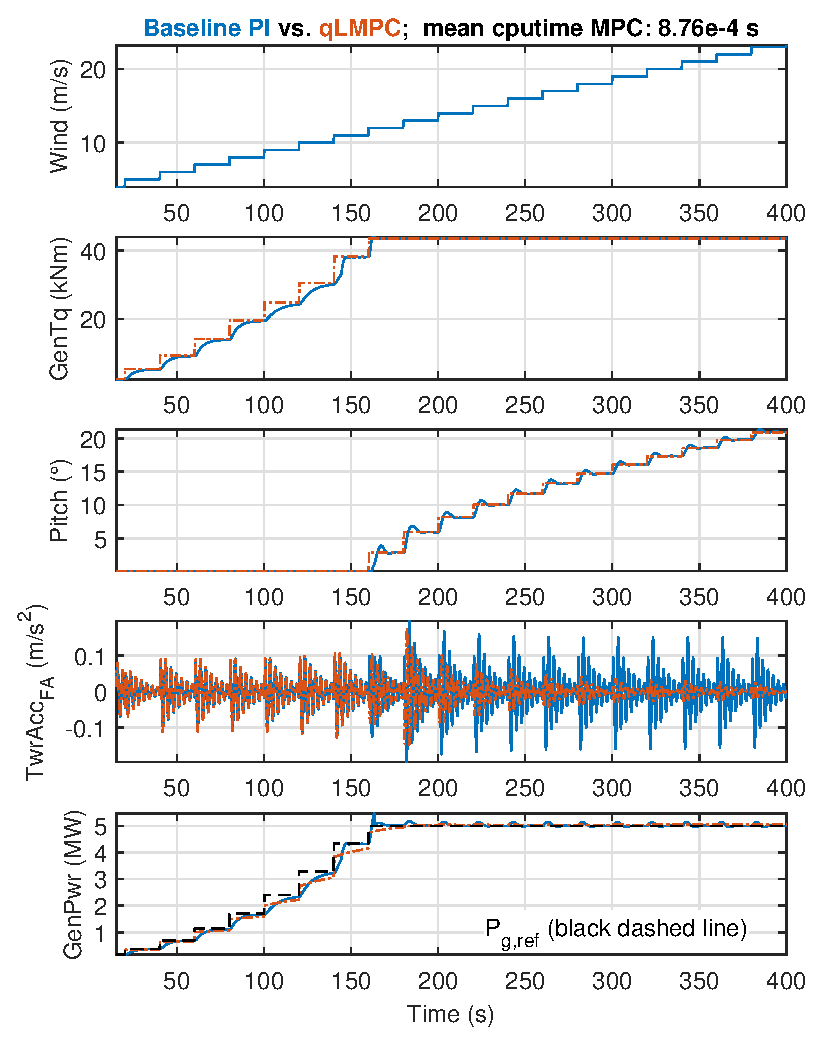
\includegraphics[width=0.485\textwidth]{figures/Figures_ADi/cmpCtrlTimeDomain_All_RefSimulinkClosedLoop_beta.eps}}\hfill 
    \subfloat[Turbulent wind, IEC class B, 18~m/s mean speed]{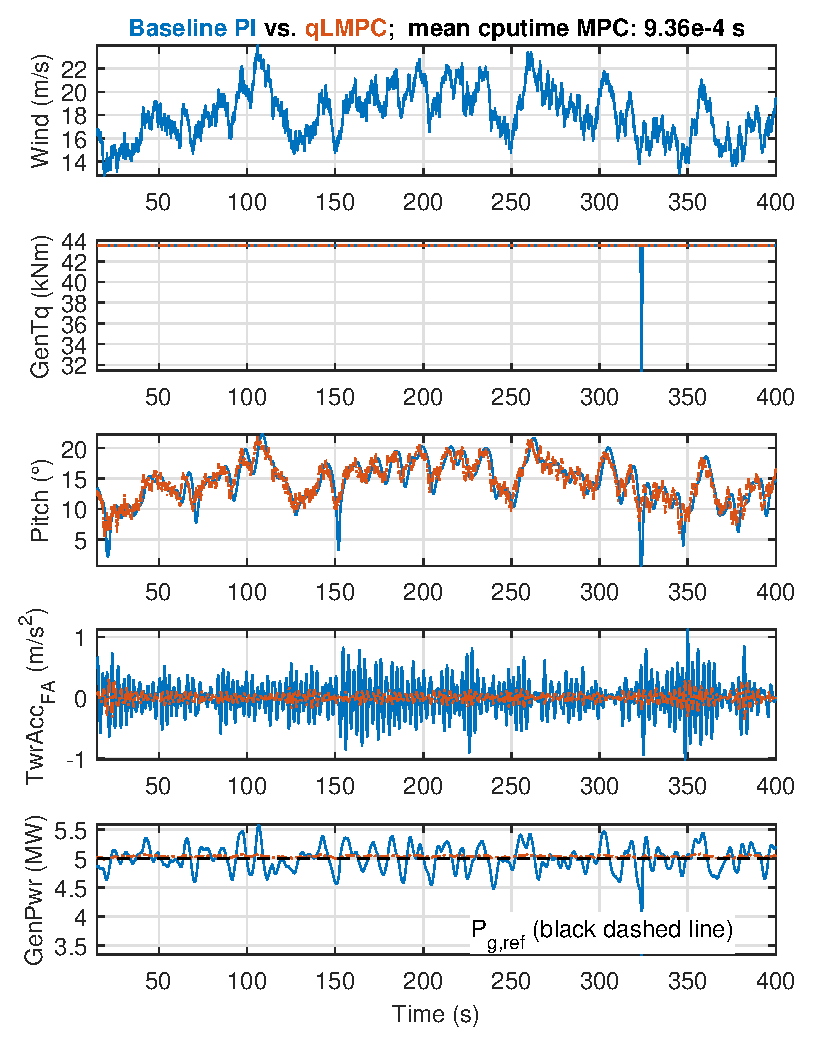
\includegraphics[width=0.485\textwidth]{figures/Figures_ADi/cmpCtrlTimeDomain_All_RefSimulinkClosedLoopNTW18_beta.eps}}\hfill
    %\subfloat[blc blc]{\includegraphics[width=0.31\textwidth]{figures/twoTurbinesGreedyOpt_2d.eps}}
    \caption[Controller comparison: qLPV model with baseline 
    PI controller vs. qLMPC for stepped wind sweep and turbulent wind.]{Controller comparison: qLPV model with baseline 
        PI controller vs. qLMPC for stepped wind sweep and turbulent wind (18\,m/s mean, IEC turbulence 
        class B (14\,\%)).  PI control (blue line), qLMPC (red line) and power reference (black dashed line). Displayed signals: wind speed, control inputs, tower fore-aft
        accelerations, and power output.}
    \label{fig:CtrlCmpMdlSweep}
\end{figure}

 The QP is solved using a linear complementary problem formulation with Lemke's algorithm \cite{cisneros2020velocity}, which enables fast convergence, as real-time capability is a critical requirement for online optimization-based control. Of the 50001 controller cycles at a sampling time of 8\,ms needed for the 400\,s simulation time, only one cycle exceeded the sampling time and only 13 exceeded 2\,ms. The mean CPU time remained considerably below 2\,ms, as shown in the subplot titles of Figure~\ref{fig:CtrlCmpMdlSweep}. These measurements were obtained in MATLAB R2021b on an Intel Core i7-11850H (2.5\,GHz, 8 cores) running Windows 10. Note that for deployment on a physical turbine, a fallback strategy would be required to handle the rare cases where the solver exceeds the sampling time. This was not implemented in this proof-of-concept, but several options exist, such as blending the last available qLMPC solution with the output of the PI feedback controller.

However, the improvements regarding the reduction of tower acceleration and power variance come at the price of higher actuation rate.
Table \ref{tab:ControllerComparisonMerged} summarizes this by displaying the afore mentioned changes in tower fore-aft acceleration and power tracking error as standard deviation for physical interpretability for both the baseline PI controller and the qLMPC algorithm.  
\begin{table}[t]
    \centering
    \caption[Standard deviation comparison: Baseline PI vs.\ qLMPC for stepped wind sweep and
    turbulent wind.]%
    {Standard deviation comparison: Baseline PI vs.\ qLMPC for stepped wind sweep and
        turbulent wind (18\,m/s mean, IEC class B).
        The standard deviations obtained with the PI controller are divided by those obtained with the qLMPC; quotients above~1 indicate improvement.} %In the turbulent wind case, both controllers operate at rated   generator torque throughout, resulting in zero torque rate standard  deviation for both
    \label{tab:ControllerComparisonMerged}
    \begin{tabular}{l rr}
        \toprule
        {Standard Deviation of} & {Stepped wind sweep} & {Turbulent wind} \\
        {Signal (unit)} & \multicolumn{2}{c}{std PI / std qLMPC =  ratio} \\
        \midrule
        Tower fore-aft acceleration ( m/s$^2$) & $0.06 / 0.03 = 1.77$ & $0.17 / 0.07 = 2.31$ \\
        Power tracking error (kW) & $169.01 / 146.26 = 1.16$ & $56.68 / 14.68 = 3.86$ \\
        Generator torque rate (kNm/s) & $0.63 / 2.36 = 0.27$ & $0 / 0 = {-}$ \\
        Blade pitch rate (\textdegree/s) & $0.22 / 0.81 = 0.27$ & $0.51 / 3.60 = 0.14$ \\
        \bottomrule
    \end{tabular}
\end{table}
%
%\\begin{tablenotes}
 %   \small
%    \item In the turbulent wind case, both controllers operate at rated 
%    generator torque throughout, resulting in zero torque rate standard 
%    deviation for both.
%\end{tablenotes}
%
Ratios above~1 indicate improvement, confirming the qLMPC reduces both tower loading and power tracking error.  But the standard deviation in rates in blade pitch increase, for the turbulent wind test case even considerably so. There is also a decrease in generator torque observed for the stepped wind test case. In the turbulent wind case, both controllers operate at rated generator torque throughout, resulting in zero torque rate standard  deviation for both. As more improvement in power variance was observed for the above rated turbulent wind, the following discussion focuses on this case.

For the results of this proof-of-concept, visualized in Figure~\ref{fig:CtrlCmpMdlSweep}, no penalty is placed on pitch actuator movement, and the pitch rate limit is set to 13\textdegree/s, which is a relatively high value. Figure~\ref{fig:CtrlCmpRates} shows the results of six test runs with different pitch rate limits: three with the baseline PI controller and three with the qLMPC algorithm. The effect of different pitch rates on the PI controller is depicted in Figure~\ref{fig:CtrlCmpRates}(a), and on the qLMPC design in Figure~\ref{fig:CtrlCmpRates}(b). The selected pitch rate limits of 4\textdegree/s, 8\textdegree/s, and 13\textdegree/s represent a range from conservative to highly responsive actuator capabilities. They were chosen to explore both realistic hardware limitations and the potential performance gains of faster actuation.

The signals shown for both investigated control algorithms are the wind speed, collective blade pitch angle, rotor speed, fore-aft tower acceleration, and generator power. It should be noted that generator torque does not change at all in this above-rated test case and is hence not shown. Under baseline PI control, increasing the pitch rate shows very little effect, as the rotor acts as a filter in this pure feedback design. In contrast, the qLMPC controller shows a considerable difference when only 4\textdegree/s pitch rate is allowed compared to the two higher rates. Allowing a pitch rate of approximately 8\textdegree/s or faster improves rotor speed regulation and reduces both tower movement and power variability by more than a factor of 3. However, it also leads to higher pitch activity.  The qLMPC reduces the variance of rotor speed, tower fore-aft movement, and power output for all rate limits, even at a  4\textdegree/s rate limit. However, the qLMPC benefits from higher pitch rates, as faster pitch response enables better disturbance rejection. The trade-off between actuator activity on the one hand and load reduction and smoother power output on the other is ultimately a design decision, which may also vary over the turbine's lifetime as the pitch bearings age.

\begin{figure}[h]
    \subfloat[Baseline PI controller]{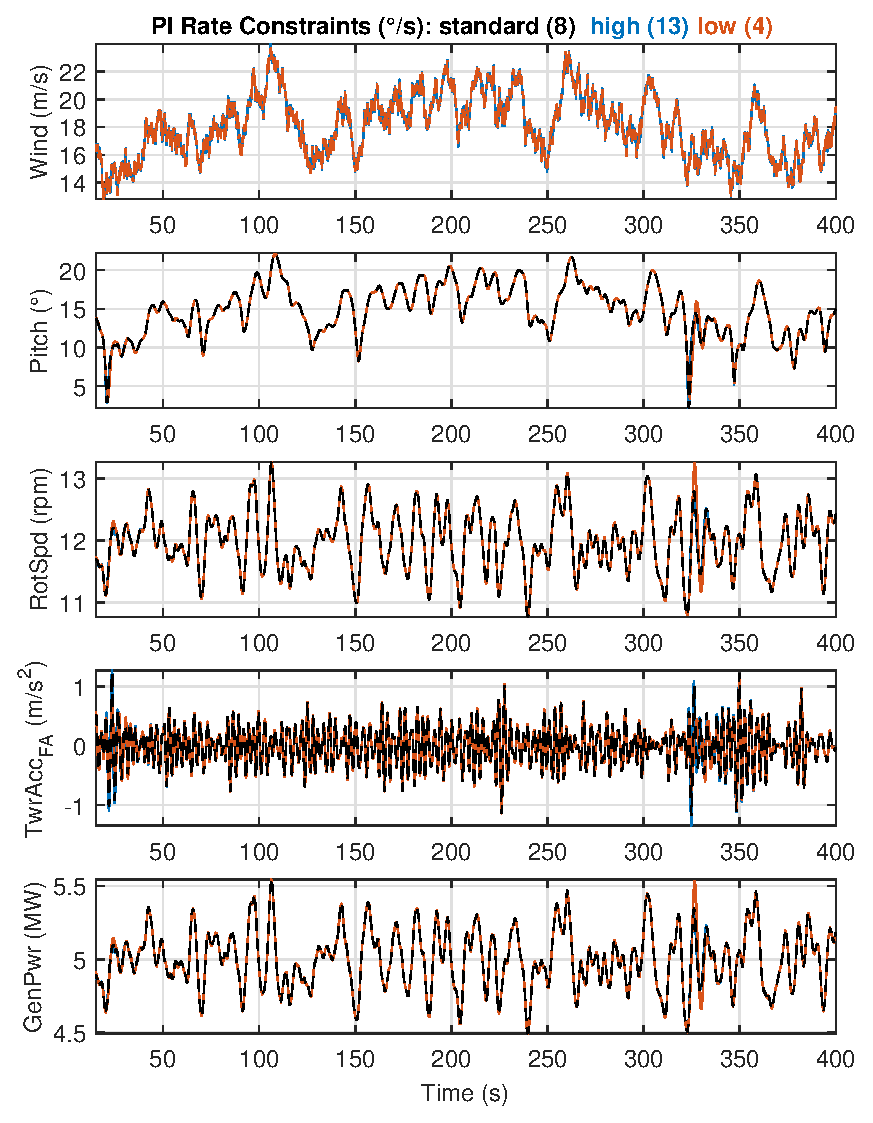
\includegraphics[width=0.485\textwidth]{figures/figDirConstr1/cmpTimeDomain_All5PINewLim.eps}}\hfill 
    \subfloat[qLMPC algorithm]{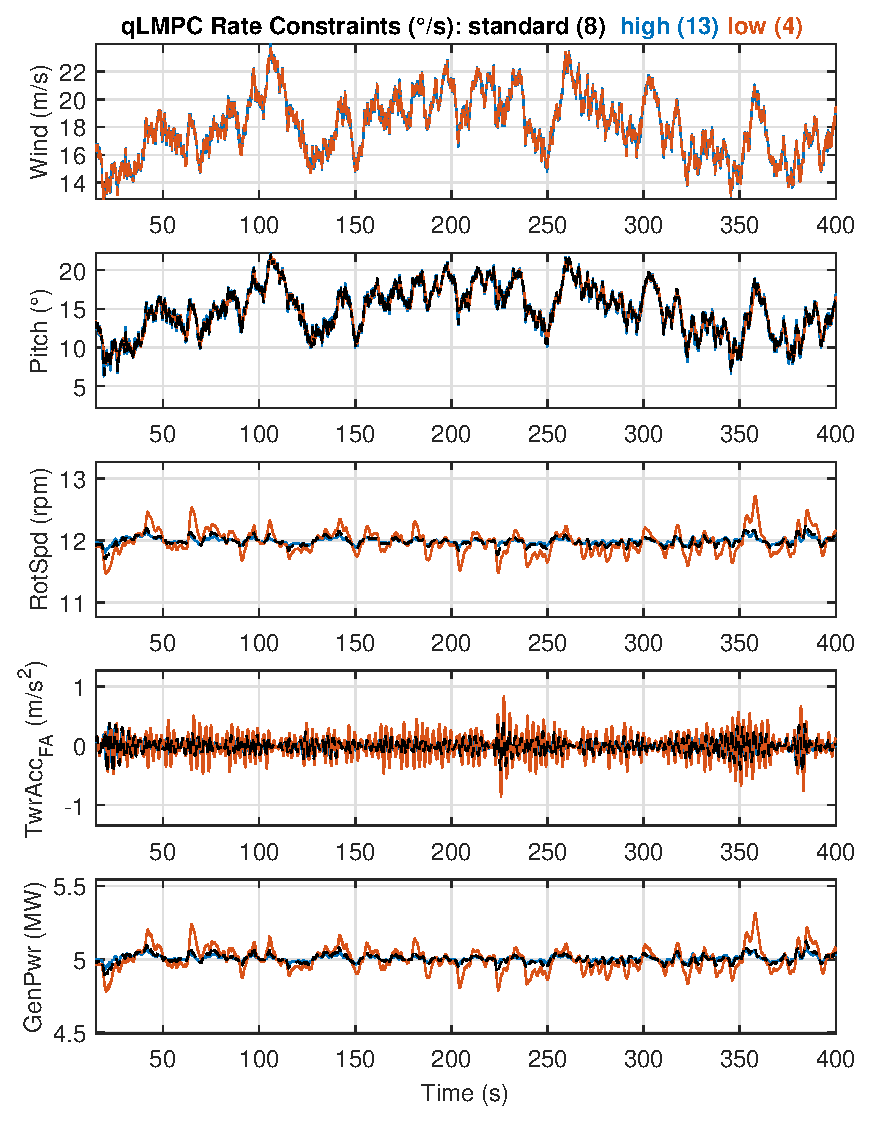
\includegraphics[width=0.485\textwidth]{figures/figDirConstr1/cmpTimeDomain_All5MPCNewLim.eps}}\hfill
     \caption[Controller comparison: Baseline PI and qLMPC with different pitch rate limits.]{Controller comparison: Baseline PI and qLMPC with different pitch rate limits for turbulent wind (18\,m/s mean, IEC turbulence  class B (14\,\%)). Rate limits: Standard 8\textdegree/s~(black line), high 13\textdegree/s~(blue line), and low 4\textdegree/s~(red line)). Displayed signals: wind speed, pitch, states, and power.}
    \label{fig:CtrlCmpRates}
\end{figure}

The standard deviations of the pitch derivative, the rotor speed, the tower fore-aft acceleration and the generated power for Figure~\ref{fig:CtrlCmpRates} are summarized in Table~\ref{tab:stddev_unified}.

\begin{table}[htbp]
    \centering
    \caption[Standard deviation comparison: Baseline PI vs.\ qLMPC for turbulent wind with different pitch rate limits.]%
    {Standard deviation comparison: Baseline PI vs.\ qLMPC
        for turbulent wind with pitch rate limits. The PI controller is largely insensitive to the rate limit
        whereas the qLMPC uses higher rates for less rotor speed, tower movement and
        power variation. Values in brackets show the ratio to the standard
        (8\,\textdegree/s) baseline PI value.}
    \label{tab:stddev_unified}
    \begin{tabular}{ll rrr}
        \toprule
        & & \multicolumn{3}{c}{Rate limit (\textdegree/s) (ratio to PI at 8\,\textdegree/s)} \\
        \cmidrule(lr){3-5}
        Controller & Signal & low: 4\textdegree/s & standard: 8\textdegree/s & high: 13\textdegree/s \\
        \midrule
        \multirow{4}{*}{PI}
        & Tower fore-aft acc.\ (m/s$^2$) & 0.32 (1.03) & 0.33 (1.00) & 0.34 (0.97) \\
        & Generated power (kW) & 200.26 (0.99) & 197.62 (1.00) & 197.32 (1.00) \\
        & Rotor speed (rpm) & 4.57 (0.99) & 4.51 (1.00) & 4.50 (1.00) \\
        & Blade pitch rate (\textdegree/s) & 1.21 (1.06) & 1.28 (1.00) & 1.34 (0.96) \\
        \midrule
        \multirow{4}{*}{qLMPC}
        & Tower fore-aft acc.\ (m/s$^2$) & 0.21 (1.57) & 0.11 (3.00) & 0.08 (4.12) \\
        & Generated power (kW) & 78.37 (2.52) & 30.72 (6.43) & 19.63 (10.07) \\
        & Rotor speed (rpm) & 1.79 (2.52) & 0.70 (6.44) & 0.45 (10.02) \\
        & Blade pitch rate (\textdegree/s) & 1.84 (0.70) & 3.11 (0.41) & 3.88 (0.33) \\
        \bottomrule
    \end{tabular}
\end{table}

The application of the proposed velocity-based qLMPC concept significantly reduces tower movements and minimizes power output fluctuations. As noted at the start of this section, DEL reduction is not directly a qLMPC objective. However, it will be shown in Section~\ref{subsection: IPCResults} and~\ref{subsec:ComparisonWindTurbineControlDesigns} that the reduced tower movement also results in considerably reduced Damage Equivalent Loads (DELs) and the corresponding values are included in comparisons with other control schemes in the Figures~\ref{fig:EvalCrit1} and~\ref{fig:CtrlCompAll}.

The performance improvement comes at the cost of requiring accurate wind information, either obtained through expensive sensors such as lidars or through wind estimations. A purely feedback-based improvement over standard collective pitch control is individual pitch control, which uses blade root moments and rotor azimuth position as additional feedback signals and is already widely deployed in commercial turbines. This approach is widely investigated in both theoretical studies and field tests and has proven to be an effective strategy, either as an alternative or in addition to MPC, to further reduce mechanical loads. While its primary focus is on reducing blade loads, a reduction in tower loads is also possible, as will be discussed in the next section.

\section{Individual Pitch Control Design and Application}\label{section:Individal Pitch PI Control}
Individual Pitch Control (IPC) is a control technique designed to mitigate cyclic loads on wind turbine blades by independently adjusting the pitch angle of each blade. These cyclic loads primarily result from wind shear, i.e., the increase in wind speed with altitude due to reduced surface friction farther from the ground. Additional causes of load imbalances include wind turbulence, gusts and tower shadow effects. These effects lead to asymmetric aerodynamic loading, causing blade movements out of the rotor plane and inducing what are referred to as out-of-plane bending moments at the blade roots. The flapwise and edgewise blade root bending moments are measured directly, for example via strain gauges. The out-of-plane bending moments are then calculated from these measured signals. They occur at specific multiples of the rotor's rotational frequency, commonly referred to as $n\text{P}$ frequencies, e.g., $1\text{P}$ and $2\text{P}$ correspond to once and twice per revolution, respectively. It is important to avoid or damp these frequencies because they can excite the turbine's natural structural modes, leading to resonant oscillations that significantly accelerate mechanical fatigue and reduce component lifespan.

The turbine blade movement can be decomposed into three primary directions relative to the blade itself, which can be measured by sensors: flapwise, which is perpendicular to the rotor plane if the blade is not pitched, edgewise within the rotor plane, and torsional twisting along the blade’s axis. Flapwise and edgewise movements can be transformed into the blade movement within the rotor plane and perpendicular to the rotor plane. The latter movements generate the aforementioned out-of-plane moments. These moments serve as feedback for IPC. IPC effectively targets and suppresses these loads by transforming the blade root moments from the rotating to the stationary rotor coordinate system, augmenting them using a controller, and then re-transforming them back into the rotating frame before applying the adjustments to the blade pitch signals.

The block diagram in Figure~\ref{fig:BlockIPC} illustrates the IPC architecture. It shows the main components of the system, including the controller, which is divided into the power controller and the IPC controller, highlighted in red. The figure also displays the NREL 5MW wind turbine, the pitch actuator, and the torque actuator.
\begin{figure}[ht]
    \centering
    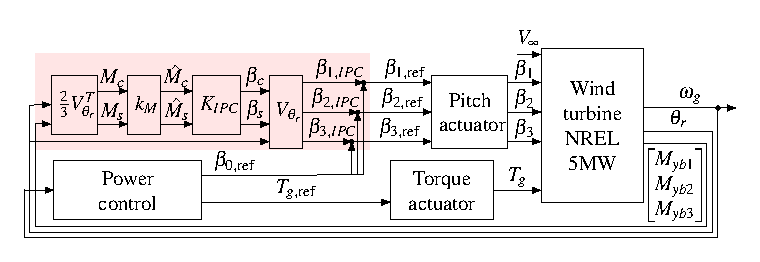
\includegraphics[width=0.9\textwidth,trim={0 0cm 0cm 0.3cm},clip]{figures/Figures_ADi/turbineCtrlBetaIPCcl.pdf}
    
     \caption[Block diagram closed-loop wind turbine control structure with IPC PI added to the baseline PI controller.]{Block diagram of the closed-loop wind turbine control structure with IPC PI (highlighted in red) added to the baseline PI controller.}
    \label{fig:BlockIPC}
\end{figure}
In this work, PI controllers are utilized rather than full PID architectures. This choice is consistent with the NREL 5MW baseline controller provided in FAST. Furthermore, numerical optimization using fminsearch for controller tuning yielded derivative gains near zero. This suggests that for the investigated load cases, the derivative action provided negligible performance improvements while potentially increasing high-frequency actuator wear due to wind turbulence noise

The three blade pitch angles $\beta_1$, $\beta_2$, and $\beta_3$ are the outputs of the pitch actuators corresponding to the references $\beta_{1,\text{ref}}$, $\beta_{2,\text{ref}}$, and $\beta_{3,\text{ref}}$. These references are the sum of the collective reference signal $\beta_{0,\text{ref}}$ from the power controller and the respective IPC adjustments $\beta_{1,\text{IPC}}$, $\beta_{2,\text{IPC}}$, and $\beta_{3,\text{IPC}}$.
%
As before, the power control loop sets the collective pitch reference $\beta_{0,\text{ref}}$ as well as the generator torque reference $T_{g,\text{ref}}$, based on feedback from the generator speed $\omega_g$.
%
These IPC adjustments are derived from the measured out-of-plane blade root bending moments $M_{yb1}$, $M_{yb2}$, and $M_{yb3}$ and the position of the first blade $\theta_{r}$, also called the rotor position or rotor azimuth. The blade root moments are transformed from the rotating into the stationary rotor coordinate system by a multiplication with the matrix $2/3 V^T_{\theta_{r}}$. The back-transformation before applying the control signals onto the rotating blades is done with a multiplication with the matrix $V_{\theta_{r}}$. The underlying method for these coordinate transformations, known as multiblade coordinate transformation, and the design of $V_{\theta_{r}}$ is explained in detail in the following section.

\subsection{Multiblade Coordinate Transformation} \label{sec:MBC}
Multiblade coordinate transformation (MBC) enables the conversion of dynamic loads from the rotating coordinate system, defined by the azimuth angle $\theta_{r}$, to a fixed tower coordinate system. Specifically, load components at the rotation frequency are transformed via the MBC to quasi-static loads. Hence, MBC allows for a more accurate assessment of the loads acting on the turbine tower and other non-rotating components. Applying MBC to convert the rotating blade root flap moments into a fixed coordinate system for a three-bladed wind turbine results in the matrix notation %Therefore, MBC facilitates an optimal calculation of the reference control signal.
\begin{equation} \label{eq:MBC}
    \left[ \begin{array}{c}
        M_0\\
        M_c\\
        M_s
    \end{array} \right] = \frac{2}{3}
    \left[ \begin{array}{ccc}
        1/2 & 1/2 & 1/2\\
        \cos(\theta_{r}) & \cos(\theta_{r} + \frac{2\pi}{3}) & \cos(\theta_{r} + \frac{4\pi}{3})\\
        \sin(\theta_{r}) & \sin(\theta_{r} + \frac{2\pi}{3}) & \sin(\theta_{r} + \frac{4\pi}{3})
    \end{array} \right]
    \left[ \begin{array}{c}
        M_{yb1}\\
        M_{yb2}\\
        M_{yb3}
    \end{array} \right], 
\end{equation}
with  $M_{ybi}$ as the out-of-plane root moment of the $i^{\text{th}}$ blade as inputs and the moments in the non-rotating system as outputs, with these moments being the symmetric load moment $M_0$, pitch moment $M_c$ and yaw moment $M_s$, as visualized in Figure~\ref{fig:BlockIPC}. The pitch and yaw moments are used to calculate two cyclic control signals $q_c$ and $q_s$, i.e., $\beta_c$ and $\beta_s$ for IPC. 
The control signal $q_i$ of the $i^{\text{th}}$ blade is calculated via the second and third columns of the inverse MBC transformation i.e. the inverse of the matrix from Equation~(\ref{eq:MBC}) %, is then used to calculate 
\begin{equation} \label{eq:inverseMBC}
    \left[ \begin{array}{c}
        q_1\\
        q_2\\
        q_3
    \end{array} \right] = 
    \underbrace{\left[ \begin{array}{ccc}
            \cos(\theta_{r}) &  \sin(\theta_{r})\\
            \cos(\theta_{r} + \frac{2\pi}{3}) &  \sin(\theta_{r} + \frac{2\pi}{3})\\
            \cos(\theta_{r} + \frac{4\pi}{3}) &  \sin(\theta_{r} + \frac{4\pi}{3})
        \end{array} \right]}_{V_{\theta_{r}}}
    \left[ \begin{array}{c}
        q_c\\
        q_s
    \end{array} \right],
\end{equation}
where the signal $q_i$ denotes $\beta_{i,\text{IPC}}$ in IPC for the $i^{\text{th}}$ blade. %In Section~\ref{sec:CombinedIPC-TrailingEdgeFlapControl} the same matrix multiplication is once again applied to the $i^{\text{th}}$ flap.
 Note that the transpose of the matrix $V_{\theta_{r}}$ from equation~(\ref{eq:inverseMBC}), multiplied by $2/3$, is equal to the last two rows of the MBC matrix, see also \cite{ossmann2017load}. In the context of this work, and as is common in related literature, see e.g.~\cite{he2018combined}, the pitch and yaw moments $M_c$ and $M_s$ are controlled via $q_c$ and $q_s$ independently, i.e., any remaining coupling following the MBC transformation between $q_c$ and $M_s$ as well as $q_s$ and $M_c$ is neglected. As the wind turbine dynamics can be modeled as a LTI system after transforming rotor blade dynamics into a fixed coordinate system, using MBC from equation~(\ref{eq:MBC}), a simple, intuitive control approach is adopted. Two separate SISO controllers, one for the blade pitch and one for the yaw moment, respectively, are designed to reduce the transformed moments $M_c$ and $M_s$. In this work, the same controller parameters are used, resulting in three parameters to be tuned for this PI controller. Similar to the IPC implementation, only PI controllers were investigated as the inclusion of a derivative component did not yield gains significantly different from zero during the tuning process. Note that the moment $M_0$, corresponding to the rotor-induced drive shaft torque and influencing generator speed and power, is controlled separately by the baseline power controller and is not used in the IPC controls. 
moments are addressed with the IPC control loop. The 2P loads are addressed with the trailing-edge flap controller making use of the fast flap dynamics.

\subsection{IPC Parameter Optimization} \label{subsection: IPCOptCriteria}
The primary objective of wind turbine control is to minimize the levelized cost of energy (LCoE) by balancing the conflicting goals of maximizing power output while minimizing mechanical loads, particularly damage equivalent loads (DELs) on the tower and blades. This work leverages controller optimization criteria originally used by \cite{hoffmann2018load}, where a standard baseline wind turbine controller, comprising generator torque control and a gain-scheduled PI pitch controller, is augmented with an IPC PI controller and tower damping. The optimization criteria in a multi-objective optimization were the minimization of blade and tower DELs, actuator dynamics, power tracking error, and standard deviation.

The PI design presented in this thesis is a two step approach: In a first step, initial values for the integral and proportional gain of the IPC are found via a grid search. Following this, the three PI parameters are optimized with the Nelder-Mead simplex algorithm implemented in MATLAB’s \textit{fminsearch.m} to reduce the blade DEL. The initial values of the proportional and integral gain are the ones previously found with the grid search. The derivative initial value is set to zero. % and found to diverge very little from it. 
For both steps of the controller tuning, the grid search as well as for the optimization, the quality of an IPC controller are quantified via the decrease in blade root DEL. The cost function $J$ to be minimized by the IPC is the maximum of the DEL of the three blades: 
\begin{equation} \label{eq:costFunIPC}
    J = \text{min}(\text{max}\left(\text{DEL}_{bi,\text{IPC}}/\text{DEL}_{\text{bi,\text{baseline}}}\right)), \quad \text{i} \in {1,2,3} 
\end{equation} %\underset{\Delta u}{\text{minimize }}
with $\text{DEL}_{bi,\text{IPC}}$ derived from the blade flapwise root DEL accumulated over a simulation run with IPC normalized by $\text{DEL}_{\text{bi,\text{baseline}}}$ with only the baseline controller active.
%\subsection{Optimization and evaluation criteria}
To evaluate and quantify the impact of an IPC controller's performance, four additional criteria are calculated, previously used in \cite{hoffmann2018load} as optimization criteria in a multi-objective optimization approach: The tower DELs derived from the bending moments at the base of the tower, the mean and standard deviation of the generated power and the additional power requirements of the actuator due to individual pitch control. The evaluation criteria can be summarized as below.

\subsubsection*{Load Criteria: Blade $C_{\text{DEL},b} = J$ and tower DEL $C_{\text{DEL},t}$}
Reducing the blade DEL is the main incentive for using IPC to decrease the Power Spectral Density (PSD) at 1P. A reduction at the 1P frequency does not influence the tower DEL, however, finding a controller that decreases the peak at 1P tends to also result in a lower PSD for a wider frequency range including the peak at 2P. Thus, a small decrease in the tower DEL is also achieved although this criterion is not included in the objective function. In Section~\ref{sec:CombinedIPC-TrailingEdgeFlapControl} it will be discussed that decreasing the PSD at the 2P frequency via the flaps does decrease the tower DELs futher. 

The blade DEL is calculated as
\begin{align*}
     \Tilde{D}_{b} &=   \frac{1}{3}  \sum_{n_b=1}^3\sum_{i=1}^{k}\left(l_{bn_b,i}  M_{yb,i}^{m_{\text{GFRP}}}\right)
\end{align*}
with $l_{b}$ as the recorded stress level and $M_{yb,i}$ as the out-of-plane root bending moment measured at the $k$ samples of a simulation run for all blades.  The Wöhler coefficient of carbon is $m_{\text{GFRP}} =10$. Note that because of this even exponent, both negative and positive moments with large amplitudes increase the damage value.
The equation for the damage criterion of the three blades is:
\begin{align*}
    C_{\text{DEL},b} &=  \Tilde{D}_{b,\text{IPC}}/\Tilde{D}_{b,\text{baseline}}  %\frac{1}{\Tilde{D}_{b,\text{baseline}}} 
\end{align*}
%
with  $\Tilde{D}_{b,\text{IPC}}$ and $\Tilde{D}_{b,\text{baseline}}$ as the recorded blade damage for the two controllers for the same test case. 

The equation for the tower damage criterion is
\begin{align*}
    C_{\text{DEL},t} &= \frac{1}{\Tilde{D}_{t,\text{baseline}}} \cdot
    \left[ \sum_{i=1}^{k_{t}} \left( l_{t,i} \cdot M_{xt,i}^{m_{\text{Steel}}} \right) + 
    \sum_{i=1}^{k_{t}} \left( l_{t,i} \cdot M_{yt,i}^{m_{\text{Steel}}} \right) \right]
\end{align*}
with $\Tilde{D}_{t,\text{baseline}}$ as the recorded tower damage for the CPC-PI controller for the same test case, $m_{\text{Steel}} =4$ the Wöhler coefficient of steel, $M_{xt,i}$ and $M_{yt,i}$ the tower moments at the top around the longitudinal and lateral axis, respectively,  $l_{t,i}$ the recorded stress level, and $k_t$ the number of data samples.

\subsubsection*{Power Criteria: Mean $C_{\bar{P}}$ and Standard Deviation $C_{\delta_P}$}
As the annual energy production should not suffer from IPC, the generated power is compared as well. It was found that the power production loss and variance increase is at 0.1\% and hence negligible. The power variance is important for the network stability, especially in small networks. The effect of the IPC controller is found to be nearly negligible. Similarly to the DEL criteria, the power criteria are normalized by the results obtained with the CPC-PI controller
\begin{align*} %\label{eq:CP}
    C_{\bar{P}} =  \bar{P}_{\text{g,\text{IPC}}}/ \bar{P}_{\text{g,\text{baseline}}}  \quad\text{and}\quad C_{\delta P} =  \delta P_{g,\text{IPC}}/ \delta P_{g,\text{baseline}}.
\end{align*} 

\subsubsection*{Actuator Power Criterion $C_{\text{Act}}$}
This is the only criterion for which an increase is unavoidable, due to the additional movement of the blades required by the IPC controller. The actuator power criterion is normalized as:
\begin{equation} \label{eq:CAct}
    C_{\text{Act}} = \frac{P_{\text{Act}, \text{IPC}}}{P_{\text{Act}, \text{baseline}}}.
\end{equation}
where \( P_{\text{Act}, \text{baseline}} \) is the reference actuator power of the baseline controller. The actuator power is defined as the mean product of the blade pitch rate $\dot{\beta}$ and the actuator pitch moments $M_{bz}$:
\begin{equation} \label{eq:CAct_calc}
    P_{\text{Act}, \text{IPC}} = \frac{1}{3} \sum_{b=1}^3 \overline{|\dot{\beta} \cdot M_{bz}|}.
\end{equation}
The controller parameters are optimized for different pitch rate limits, as the optimization objectives described above converge to different optima depending on the actuator constraints. As in the analysis of the qLMPC controller behavior, the rates are set to 4\textdegree/s, 8\textdegree/s, and 13\textdegree/s to investigate settings ranging from very conservative to highly agile. In the following results section, a comparative analysis in both the time and frequency domains is presented to illustrate how these trade-offs affect structural loads, power output, and actuator behavior, i.e., the quantitative controller objectives described in this section.

\subsection{Results} \label{subsection: IPCResults}
Figure~\ref{fig:timeseriesIPC} visualizes the results of the baseline CPC and two IPC controllers, with parameters optimized for 4\,m/s and 13\,m/s pitch rate limits. In all test cases, the turbine is excited with the same wind signal, which has a mean wind speed of 16\,m/s and corresponds to turbulence class B. The first subplot shows this wind speed signal, which is also used for controller tuning during the optimization. The subsequent plots display generator torque, pitch angles, rotor speed, tower fore-aft acceleration, generator power, and blade root out-of-plane moments.
\begin{figure} [H]
    \subfloat[Pitch rate limit 4\textdegree/s]{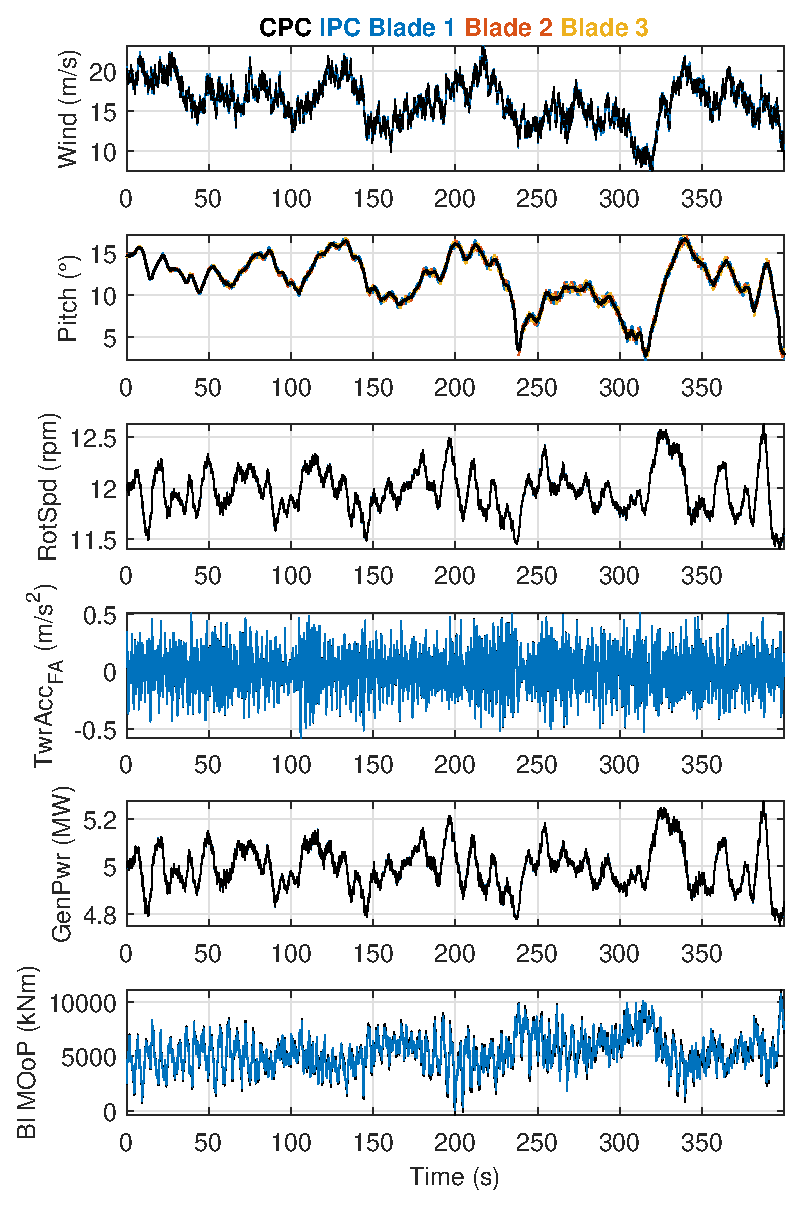
\includegraphics[width=0.49\textwidth]{figures/figures_WESC25/fig00a_Timeseries1.eps}}\hfill 
    \subfloat[Pitch rate limit 13\textdegree/s]{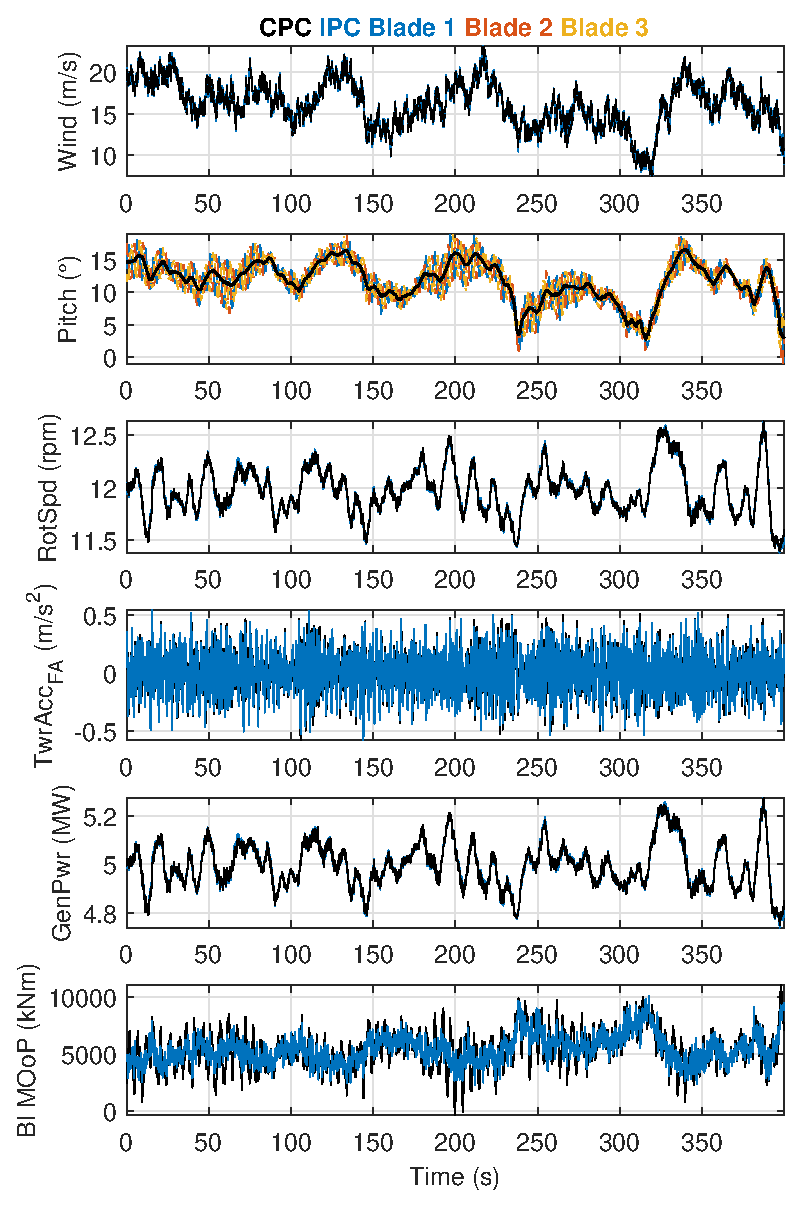
\includegraphics[width=0.49\textwidth]{figures/figures_WESC25/fig00a_Timeseries3.eps}}\hfill
    \caption[Controller comparison: Baseline and IPC PI with different pitch rate limits.]{Controller comparison: Baseline (black) and IPC PI (blue, red and yellow lines pitch signals, blue all other signals) with different pitch rate limits for turbulent wind (16\,m/s mean, IEC turbulence class B (14\,\%)). Rate limits: Low (4\textdegree/s) and high (13\textdegree/s~) for IPC, standard  (8\textdegree/s) for baseline PI. Displayed signals: wind speed, pitch, states, power, and out-of-plane blade root moments.}
    \label{fig:timeseriesIPC}
\end{figure}

Generator torque, rotor speed, and generator power remain nearly unchanged between the two IPC configurations and the baseline PI CPC. This is expected, as the power control logic, which sets the generator torque and collective pitch demand, is identical across all controllers. Differences in tower fore-aft motion are also nearly imperceptible in this time series. The most notable differences appear in the pitch signals, which oscillate at the 1P frequency in both IPC cases, and in the resulting blade root out-of-plane moments. At the lower pitch rate limit of 4\textdegree/s, shown in the left column, the IPC controller has also only a limited effect on the blade root out-of-plane moments. In contrast, the right column, corresponding to the very high pitch rate limit of 13\textdegree/s, shows that the individual pitch actuators significantly reduce the variance of the out-of-plane moments, thereby improving load reduction on the blades. A very slight decrease in tower fore-aft acceleration is also detectable at this rate limit. 
As expected, increasing the allowable pitch rate enhances the effectiveness of the IPC controller in alleviating structural loads.   

Figure~\ref{fig:PSDIPC} shows the Power Spectral Density (PSD) of the blade root out-of-plane moment to visualize and explain the gradual improvement with increasing pitch rate for all three test cases. The black line represents the baseline CPC. The blue line, representing IPC with a 4°/s rate limit, reduces the 1P peak by 87\%, while the red line, representing IPC with an 8°/s rate limit, further lowers it, achieving a significant 98\% reduction. At the 2P frequency, the blue line shows a slight increase compared to the baseline, while the red line effectively lowers the 2P peak. As expected, the 8°/s rate limit offers better load reduction across both 1P and 2P frequencies. The controller tuned with the rate limit set to 13°/s, depicted as a yellow line, decreases the 1P and 2P peaks even more. 
\begin{figure}[h]
    \begin{center}
        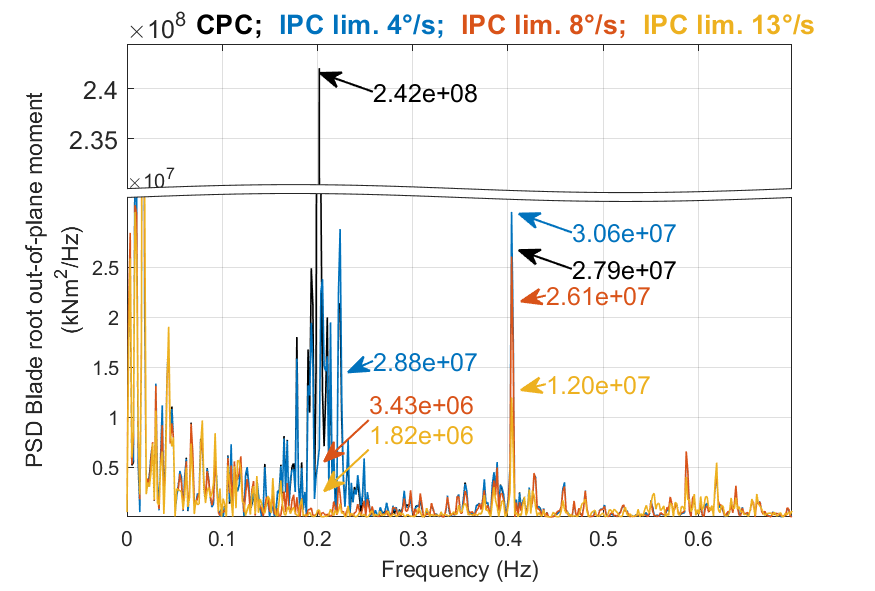
\includegraphics[width=0.6\textwidth]{figures/figures_WESC25/fig02_PSDroot_breaky_ratecomp.png}
        \caption[Controller comparison: Power Spectral Density of blade root out-of-plane moment of baseline PI with 8\textdegree/s rate limit, IPC with 4°/s,  8°/s, and 13°/s rate limit]{Controller comparison: Power Spectral Density of blade root out-of-plane moment of baseline PI (black) with 8\textdegree/s rate limit, IPC with 4°/s rate limit (blue),  8°/s rate limit (red), and 13°/s rate limit (yellow)}
        \label{fig:PSDIPC}
    \end{center}
\end{figure}

Table~\ref{tab:stddev_unified_IPC} summarizes the standard deviation of the signals shown in Figure~\ref{fig:timeseriesIPC} for IPC rate limits of 4°/s, 8°/s, and 13°/s. The baseline PI values are completely insensitive to the rate limit as the pitch rates stay below the limit of 4°/s, they are constant across all three cases. For the states and power output, the introduction of IPC also does not produce any observable effect. Even the tower fore-aft acceleration, which appeared marginally improved under visual inspection at 13°/s, shows a ratio of 1.00 throughout. The pitch rate standard deviation increases unavoidably for the IPC test cases: by 27\% at the most restrictive limit of 4°/s, and by factors of 3.61 and 5.74 at 8°/s and 13°/s respectively. In contrast, the blade root out-of-plane moment is reduced by 5\%, 21\%, and 23\% across the three limits, consistent with the spectral load reductions at 1P and 2P visible in Figure~\ref{fig:PSDIPC}.
\begin{table}[htbp]
    \centering
   \caption[Standard deviation comparison: Baseline PI vs. IPC for turbulent wind with 
   different pitch rate limits.]{Standard deviation of IPC blade pitch rate and blade root 
       OoP moment for turbulent wind with different pitch rate limits. Values in brackets show 
       the ratio to the PI baseline. Tower fore-aft acceleration, generated power, and rotor 
       speed standard deviations are identical to the PI baseline across all rate limits and are 
       therefore omitted. PI baseline standard deviations differ only for the blade pitch rate (0.54\,\textdegree/s)
       and blade root OoP moment (1628.85\,kNm).}
    \label{tab:stddev_unified_IPC}
    \begin{tabular}{l rrr}
        \toprule
        & \multicolumn{3}{c}{ IPC rate limit (\textdegree/s) (ratio to CPC rate limit (\textdegree/s))} \\
        \cmidrule(lr){2-4}
        Signal & low: 4\textdegree/s & standard: 8\textdegree/s & high: 13\textdegree/s \\
        \midrule
        Tower fore-aft acc.\ (m/s$^2$)  & 0.17 (1.00) & 0.17 (1.00) & 0.17 (1.00) \\
        Generated power (kW)             & 91.59 (1.00) & 91.78 (1.00) & 91.97 (1.00) \\
        Rotor speed (rpm)                & 2.09 (1.00) & 2.09 (1.00) & 2.10 (1.00) \\
        Blade pitch rate (\textdegree/s) & 0.69 (1.27) & 1.95 (3.61) & 3.09 (5.74) \\
        Blade root OoP moment (kNm)      & 1546.19 (0.95) & 1282.12 (0.79) & 1248.97 (0.77) \\
        \bottomrule
    \end{tabular}
\end{table}


Figure~\ref{fig:EvalCrit1} shows the evaluation criteria, described in Section~\ref{sec:quasi-LPVTurbineModel}, for the PI IPC and the qLMPC CPC under varying pitch rate limits for the test case pictured in Figure~\ref{fig:timeseriesIPC}.  The criteria are obtained by normalizing all objectives by the values achieved with the PI
baseline for the same test case. The bar plot illustrates five performance metrics: blade
and tower damage equivalent loads $C_{\mathrm{DEL},b}$ and $C_{\mathrm{DEL},t}$, mean
power tracking error $C_{\bar{P}}$, power output standard deviation $C_{\delta_{P}}$, and
pitch actuation energy $C_{\text{Act}}$. 
Note that the standard deviation metrics used previously are insensitive to the amplitude and frequency distribution of load cycles.
DELs, which are computed via rainflow counting, capture these effects directly and are
therefore used as the performance metric for mechanical loads throughout the remainder of
this section. With IPC, blade root DELs are reduced by 3\%, 14\%, and 15\% depending on the pitch
rate limit, while tower DELs decrease by 3\% and 5\% at the two higher rate limits.
%\begin{figure}[htbp]
%    \begin{center}
%        \subfloat[IPC]{\includegraphics[width=0.48\textwidth]{figures_WESC25/afig01_IPCbar.eps}}\hfill
%        \subfloat[MPC]{\includegraphics[width=0.48\textwidth]{figures_WESC25/afig03_MPCbar.eps}}\hfill
%        \caption{Power criteria, actuator energy, blade and tower DEL of PI IPC and MPC CPC
%            controllers.}
%        \label{fig:EvalCrit1}
%    \end{center}
%\end{figure}

\begin{figure}[h]
    \begin{center}
        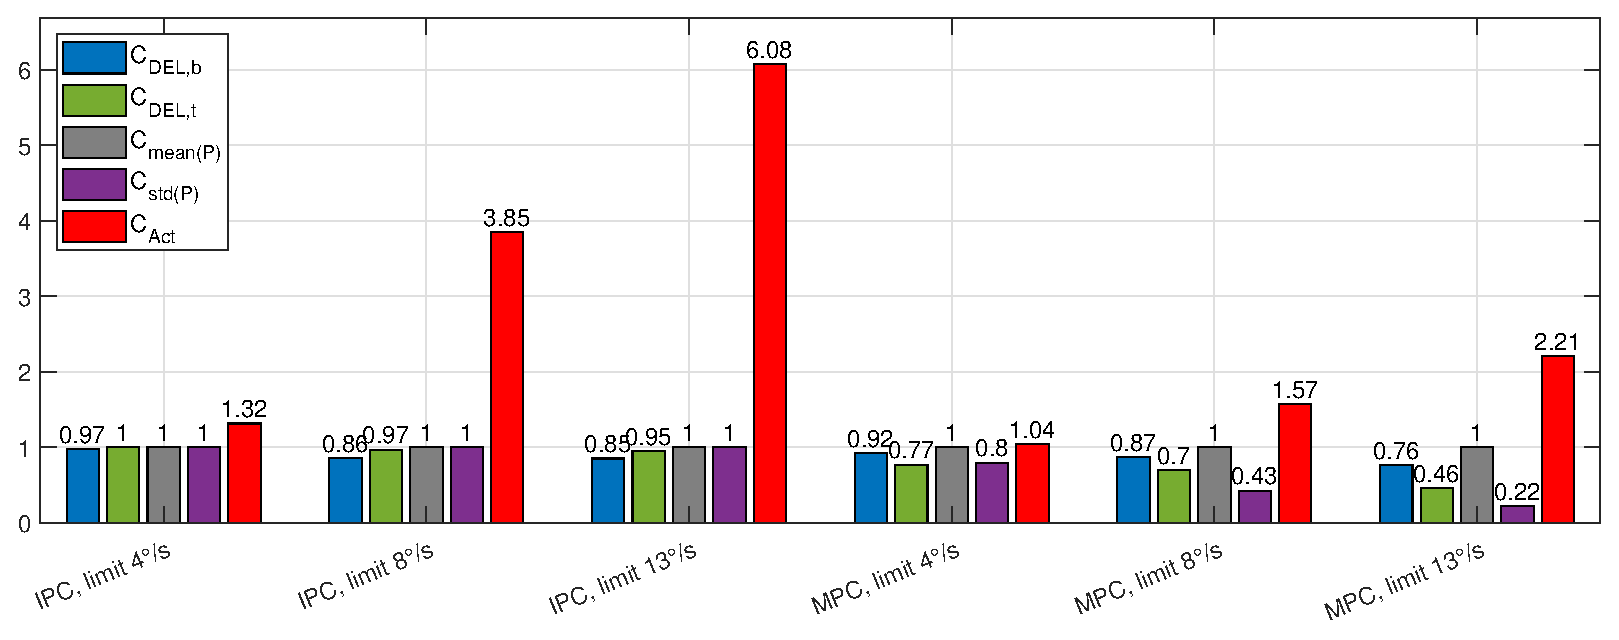
\includegraphics[width=0.95\textwidth]{figures/figures_WESC25/afig01_IPCMPCbar.eps}
        \label{tabCtrlcomp}
            
         \caption[Wind turbine controller evaluation criteria for qLMPC and IPC with different pitch rate limits for turbulent wind] {Wind turbine controller evaluation criteria  qLMPC and IPC  for turbulent wind (16\,m/s mean, IEC turbulence class B (14\%)). Criteria are tower base and blade DELS, power mean and standard deviation, and pitch actuator power.}
        \label{fig:EvalCrit1}
    \end{center}
\end{figure}



The power tracking and variance performance $C_{\bar{P}}$ and $C_{\delta_{P}}$ remain
identical to the baseline. The progressive improvement of the load reduction metrics
$C_{\mathrm{DEL},b}$ and $C_{\mathrm{DEL},t}$ with higher pitch rate limits comes at the
cost of increased pitch activity, as reflected in the strongly increasing $C_{\text{Act}}$
values of 1.32, 3.85, and 6.08. The qLMPC controller shows the same trade-off between actuator activity and load
reduction. Since the individual blade loads driven by wind shear across the rotor are not
directly addressed by collective pitch control, the stronger load reduction is observed in
the tower DEL, which is substantially reduced by 23\%, 30\%, and 54\% across the three
rate limits, reflecting the qLMPC's effectiveness in attenuating tower fore-aft motion.
While the blade DEL reductions are smaller, they are at 8\%, 13\%, and 24\% still either
larger or nearly equal to those obtained at the same pitch rate limits with IPC. As with
IPC, the power tracking performance $C_{\bar{P}}$ is not changed. However, due to the
reduction in rotor speed deviations achieved with the qLMPC, the power standard deviation
$C_{\delta_{P}}$ decreases markedly at higher rate limits, consistent with the previously
reported smoother power output. At higher pitch rate limits, the qLMPC shows an increase
in pitch activity, but significantly less so than for the IPC controller at the same
limits.

IPC was shown in this section to reduce blade loads, with the amount of reduction progressively increasing with higher pitch rate limits, at the cost of increased actuator energy. It was also shown to decrease tower loads to a certain degree. 
However, the qLMPC, discussed in the previous section, reduces tower loads more effectively, as it directly controls the collective pitch to lower thrust fluctuations. Notably, the qLMPC also achieves comparable or 
better blade load reductions than IPC, even though it does not explicitly target 
individual blade loads and based on this single time series analysis, the qLMPC appears to 
be the more effective single controller overall. However, it should be taken into account that the performance of the MPC strongly depends on the model quality as well as the agreement between estimated wind and true wind. Obviously, the performance of IPC also depends on the quality of the blade root out-of-plane measurements. Nevertheless, IPC Pi controllers are at the moment more widely accepted as a relatively simple method for larger turbines to decrease blade loads. An MPC IPC approach could reduce blade and tower loads even further, but the combined actuator demand may become 
unacceptably high.

While this section focused on load mitigation through individual pitch control, further 
improvements can be achieved by including additional actuators. As blade sizes continue to 
increase, additional actuation devices integrated into the blade structure might become 
necessary. The following section introduces a turbine model enhanced 
with trailing edge flaps on the rotor blades, enabling combined IPC and flap control for 
more effective high-frequency load reduction.

\section{Combined IPC Trailing Edge Flap Control Design and Application}
\label{sec:CombinedIPC-TrailingEdgeFlapControl}

Building on the previous investigations into IPC and qLMPC strategies, this section focuses on a combined control approach that incorporates both IPC and Trailing Edge Flaps (TEF). By including TEFs in the rotor blades as supplementary actuation surfaces, additional degrees of freedom become available for targeted load mitigation, particularly at higher frequencies. This combination of individual pitch and trailing edge flap control is referred to as IPC-TEFC or Active Aerodynamic Load Control (AALC). AALC is defined as the integrated use of multiple aerodynamic control surfaces to actively reduce structural loads and improve turbine performance. By coordinating both individual blade pitch adjustments and trailing edge flap deflections, AALC provides enhanced load mitigation compared to each method alone. This section presents the model formulation for incorporating TEFs into the wind turbine dynamics and evaluates a combined IPC–TEFC strategy across Region~III operation. The controller design is based on an optimization framework that considers multiple wind conditions and turbulence intensities to ensure good performance over the whole operating range. Following the methodology outlined in the report \cite{osterwinter2019load1}, the approach is validated using a comprehensive set of verification wind fields to assess load reduction, power preservation, and actuator demand. This work has been published in \cite{dittmer2024combined}.


\subsection{TEF Simulation Model} %bonnie_jonkman_openfastopenfast_2022 OpenFAST2023
As before, the OpenFAST simulation software is used to investigate the benefits of combining individual pitch and trailing-edge flap control. The NREL 5MW wind turbine model is modified to implement controllable trailing-edge flaps on the rotor blades. The original NREL 5MW model without TEF serves as a reference for analyzing the aerodynamic effects of these modifications on the simulated operation of the turbine. 
\subsubsection*{Rotor Blade Geometry and Aerodynamics}
The rotor blades of the NREL 5MW turbine are defined by eight distinct cross-sectional profiles distributed along the blade length, as illustrated in Figure~\ref{subfig:TEF1}, and comprise 19 nodes, each with specific geometric profile shapes. At the root, cylindrical profiles connect to the rotor hub, accommodating high bending moments and pitch adjustments. The profiles transition from the DU series, developed at Delft University of Technology, near the root to the NACA64 profile in the outer 29\% of the blade, characterized by decreasing thickness towards the tip. The blade's aerodynamic efficiency is further refined by varying the profile depth and orientation at each node.

The blade section with trailing-edge flaps, which covers the whole NACA64 blade section, is marked in red. The flap-to-blade chord ratio amounts to 20\%. The aerodynamic model of the blade enhanced with TEF requires input data on lift, drag, and pitching moment coefficients for all profiles across various blade angles of attack and a variety of flap deflection angles. The three main factors influencing these aerodynamic properties are surface roughness, Mach number, and Reynolds numbers. The OpenFAST simulation neglects surface roughness variations due to contaminants. The airflow is assumed to be incompressible with a Mach number of 0.25 at the blade tip. Interpolating between different polars is implemented in OpenFAST based on a user-defined parameter, by default the Reynolds number. In this work the interpolation between polars is performed based on the flap positions. As only one interpolation parameter can be defined, the Reynolds number distribution depicted in Figure~\ref{subfig:TEF1} is used for all wind speeds. Care was taken to model the distribution of Reynolds numbers along the rotor blade at this wind speed as realistically as possible. Realistic Reynolds numbers for rotor blades range from one to eight million are obtained from an OpenFAST simulation with turbulence class A at a mean wind speed of 12\,m/s. The OpenFAST aerodynamic models of the rotor blades are extended with additional airfoil polars based on this distribution.  % with the numbers obtained via an OpenFAST simulation run with a wind file from the optimization data set, with turbulence class A and the meand wind speed at 12\,m/s.
\begin{figure}[h]
    \centering
    \includegraphics[width=0.6\textwidth]{Images_Torque24/fig01_RE.eps}\hspace{0pc}%
    \begin{minipage}[b]{0.95\textwidth}\caption[ Span-wise distribution of Reynolds numbers Re at wind speed $V_{\infty} = 12$\,m/s]{\label{subfig:TEF1} Span-wise distribution of Reynolds numbers Re at wind speed $V_{\infty} = 12$\,m/s (from OpenFAST simulation) and blade geometry with cylinder, DU40, DU35, DU30, DU25, DU21 and NACA64 profiles with TEF location covering the NACA64 section marked in red.}
    \end{minipage}
\end{figure}

\subsubsection{Polar Calculation with xflr5 and XFOIL}
The aerodynamic coefficients of rotor blade profiles for the TEF enhanced blades are calculated using the programs xflr5 and XFOIL, see \cite{drela1989xfoil}. XFOIL uses a higher-order panel method to analyze and design airfoil profiles, incorporating variables like Reynolds number, Mach number, and a transition criterion for calculating the shift from laminar to turbulent flow. The turbulence degree of the incoming flow determines the appropriate transition criterion value, with the default value set at 9, approximating a median turbulence level as per XFOIL's documentation. For fluid properties, standard sea-level values from the International Standard Atmosphere (ISA) are used. The aerodynamic coefficients for the respective profiles are calculated based on the Reynolds numbers selected from Figure \ref{subfig:TEF1}. The coefficients generated by xflr5 and XFOIL are not directly suitable for wind turbine simulation as AeroDyn15 requires coefficients over an angle of attack range from -180\textdegree{} to +180\textdegree. Since XFOIL's panel methods yield accurate results only up to the point of flow separation, the polars are extrapolated to cover the entire required angle range. This extrapolation is performed using the AirfoilPrep preprocessor developed by NREL, applying the Viterna method for extrapolating polars, see for details e.g.~\cite{gasch2011wind}. %on Viterna's calculation process 
Additionally, corrections are made to account for three-dimensional flow effects caused by the rotor blade's rotation. Factors like Coriolis and centrifugal forces increase the maximum lift coefficients in the inner rotor areas. These 3D effects are corrected using functions integrated into AirfoilPrep. Figure \ref{subfig:TEF2} illustrates the extrapolated and corrected lift and drag coefficients over the angle of attack for rotor blade profiles with different flap angles. 

Figure \ref{subfig:TEF2}\,(a) shows that a positive flap deflection leads to an increase in lift coefficients $c_l$ and hence in lift. A positive flap deflection is defined as the flap moving backwards with respect to the chord line of the local blade profile with an undeflected flap. The point of maximum lift coefficient shifts to a smaller angle of attack than with a neutral flap position. A negative flap deflection has the opposite effect. The lift coefficients are reduced and the point of maximum lift coefficient shifts to higher angles of attack. This corresponds to the expected effects of different trailing-edge flap deflections on the lift. 

Figure~\ref{subfig:TEF2}\,(b) visualizes the drag coefficient. The curves of the drag coefficient $c_d$ appear smooth and physically meaningful for angles of attacks above -27\textdegree. Note that there is a sudden reversal of the vertical staggering of the polars below this value. There is neither a physical explanation for this effect, nor is any discontinuity observed for the rotor profile without trailing-edge flap. It can be assumed that the extrapolation method does not work optimally for profiles with flaps at these high TEF angles that would lead to flow separation and stall.  However, this can be disregarded as the range of TEF angles of attack in the simulations in the outer area of the rotor blades do not exceed -27\textdegree\ during normal operation. As this study uses OpenFAST v3.2.1, no additional code needs to be added for the TEF inclusion, unlike earlier studies that leveraged previous versions of FAST. The obtained coefficients are summarized in a text file, which is included as a parameter in the Airfoil Information section of the AeroDyn15.dat file of the NREL 5MW model available in the Git repo \cite{GitRepoCodeAALC}. %NACA64_A17_Flap.dat
%
\begin{figure} [h]
    \subfloat[Lift coefficient $c_{l}$]{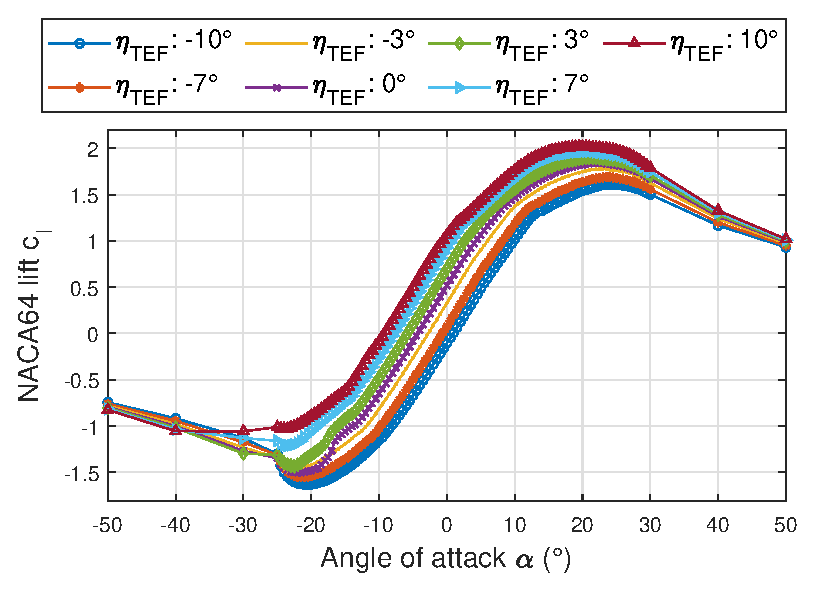
\includegraphics[width=0.485\textwidth]{figures/Images_Torque24/fig01_Cl1out.eps}}\hfill 
    \subfloat[Drag coefficient $c_{d}$]{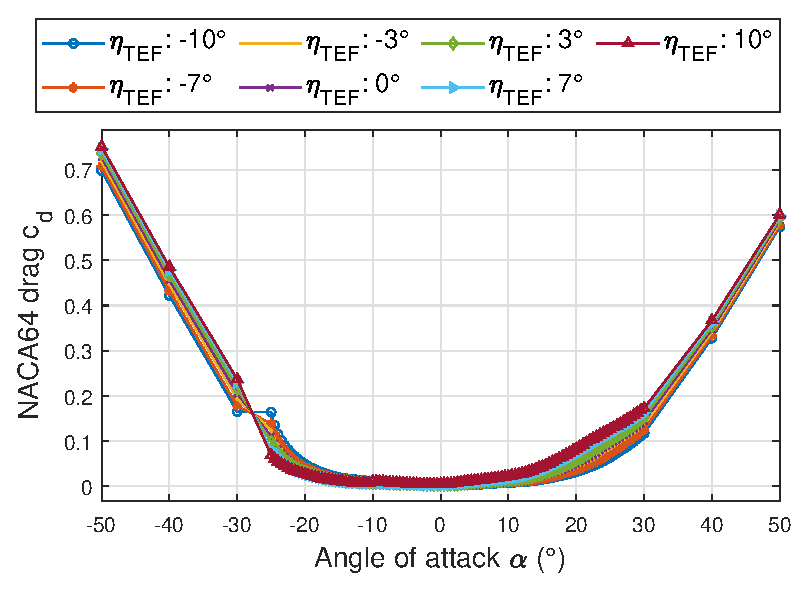
\includegraphics[width=0.485\textwidth]{figures/Images_Torque24/fig01_Cd1out.eps}}\hfill
    %\subfloat[blc blc]{\includegraphics[width=0.31\textwidth]{figures/twoTurbinesGreedyOpt_2d.eps}}
    \caption{Lift and drag coefficients at different TEF angles $\eta_{\text{TEF}}$ and different blade angles of attack $\alpha$.}
    \label{subfig:TEF2}
\end{figure}
%

\subsection*{Baseline Power Controller} %speed-controlled-pitch-controlled
In order to realistically simulate a modern turbine, a control system controlling rotor speed and generator torque is required, and the same baseline controller described and applied in the previous sections is utilized for that purpose. The aim of the IPC-TEFC is to further decrease the mechanical loads. Note that this load reduction controller using IPC together with TEF-control is an add-on controller to the baseline control system. This is possible as cyclic pitch motions are induced, which are effectively decoupled from the collective pitch motion ensuring the maximum power output above rated wind speed. As before, the implementation of the baseline controller is the power controller available within TU Delft's FASTTool, see \cite{mulders2020wind}. 
%
\subsubsection*{Open-Loop TEF Model Verification with FAST} % with TEF open loop control
The modified NREL 5MW turbine model presented in the previous section is tested in open-loop simulations with regard to the plausibility of the influence of the TEF position on the simulation results. The aerodynamic model of the trailing-edge flap is included. Open-loop control inputs of the TEF deflection angle $\eta$ are analyzed in order to investigate its suitability with regard to the desired DEL reduction. The effects of flap deflections on different parameters relevant to the operational quality of the wind turbine, such as forces and moments as well as power yield, are investigated. Figure \ref{fig:OLdiag} shows a block diagram to illustrate the control structure used for these verification tests, with the eight inputs, i.e., the seven control inputs and the wind of the selected test case $V_{\text{TC}}$ as a disturbance. The actuators for the pitch angle adjustment of the rotor blades are modeled as first order transfer function with position and rate limitations. The influences of different TEF positions for steady-state operating conditions are discussed in Section~\ref{subsec:ResultsTEF}. 
% For a sensitivity study of the flaps with regard to their influence on the blade root flapping moments, we refer to \cite{osterwinter2019load1}.
\begin{figure}[h]
    \centering
    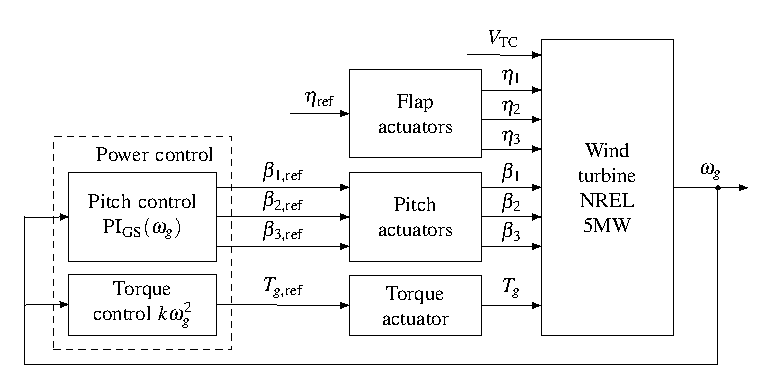
\includegraphics[width=0.95\textwidth, trim=0 0 0 13, clip]{figures/Images_Torque24/blockdiagram_OL_latex_tau2.pdf}\hspace{2pc}%
    \begin{minipage}[b]{0.95\textwidth}\caption{\label{fig:OLdiag} Block diagram for open-loop TEF verification tests with baseline power control in closed loop and open-loop collective TEF control inputs.}
    \end{minipage} %BlockschaltbildopenLoop1.jpg
\end{figure}

\subsection{IPC-TEFC Implementation}
The main design objective of the presented AALC is the reduction of structural moments, focusing on flapwise blade root bending moments. The overall controller layout is shown in Figure~\ref{fig:CLdiag}. The baseline controller, depicted in Figure~\ref{fig:OLdiag}, is enhanced with IPC, with the individual pitch demand added to the collective pitch reference, as well as TEFC which changes the TEF position. All six AALC control output signals are calculated via MBC, see Section \ref{sec:MBC}, based on the three out-of-plane blade root moments, $M_{yb1}$, $M_{yb2}$, and  $M_{yb3}$, as well as the rotor azimuth $\theta_r$. This section reviews the allocation of IPC and TEFC signals and then discusses the design of these controllers. 
\begin{figure}[h]
    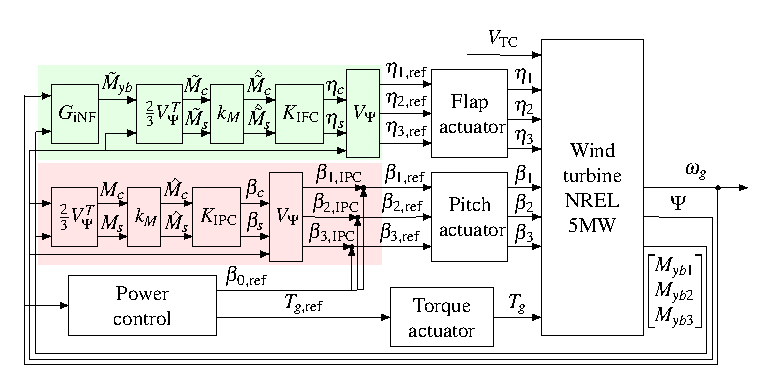
\includegraphics[width=0.95\textwidth]{figures/Images_Torque24/blockdiagram_CL_latex2.pdf}\hspace{2pc}%
    \begin{minipage}[b]{0.95\textwidth}\caption[Block diagram for closed-loop TEF verification tests with baseline power control, individual pitch and TEF closed loop control.]{\label{fig:CLdiag} Block diagram for closed-loop verification tests with baseline power control, individual pitch (highlighted in red) and TEF (highlighted in green) closed loop control.}
    \end{minipage}
\end{figure}
\subsubsection*{IPC and TEFC Control Allocation}
MBC enables the conversion of dynamic loads from the rotating blade coordinate system, defined by the azimuth angle $\theta$, to a fixed tower coordinate system. Specifically, load components in the 1P frequency range are transformed via the MBC to quasi-static loads. Hence, MBC allows for a more accurate assessment of the loads acting on the turbine tower and other non-rotating components. Applying MBC to convert the rotating blade root flap moments into a fixed coordinate system for a three-bladed wind turbine results in the matrix calculation in Equation~\eqref{eq:MBC} Therefore, MBC facilitates an optimal calculation of the reference control signal.

Figure~\ref{fig:CLdiag} denotes $M_{ybi}$ as the flapwise blade root moment of the $i^{\text{th}}$ blade as inputs, and the blade tilt moment $M_c$ and yaw moment $M_s$ in the non-rotating system as outputs. The moments $M_c$ and $M_s$ are used to calculate two cyclic control signals $q_c$ and $q_s$, i.e., $\beta_c$ and $\beta_s$ for IPC, and $\eta_c$ and $\eta_s$ for TEFC. The control signal $q_i$ of the $i^{\text{th}}$ blade is calculated via the inverse MBC transformation in Equation~\eqref{eq:inverseMBC} 
where the signal $q_i$ denotes $\beta_{i,\text{IPC}}$ and $\eta_{i,\text{ref}}$ in IPC and TEFC, for the $i^{\text{th}}$ blade or flap, respectively.  As for the IPC scheme, the tilt and yaw moments $M_c$ and $M_s$ are controlled via $q_c$ and $q_s$ independently, i.e., any remaining coupling following the MBC transformation between $q_c$ and $M_s$ as well as $q_s$ and $M_c$ is neglected. As the wind turbine dynamics can be modeled as a LTI system after transforming rotor blade dynamics into a fixed coordinate system, using MBC from Equation~(\ref{eq:MBC}), a simple, intuitive control approach is adopted. Four separate SISO controllers, two for IPC and TEFC, respectively, are designed to reduce the transformed moments $M_c$ and $M_s$. The system is now over-actuated, i.e., two moments, $M_c$ and $M_s$, need to be mitigated, but four control inputs, $\eta_c$, $\eta_s$, $\beta_c$, and $\beta_s$, are available. This offers the possibility of a frequency separation as a form of control allocation. To achieve this frequency separation of IPC and individual flap control inverse notch filters are implemented in the AALC controller. The 1P loads in the frequency spectrum of the blade root bending moments are addressed with the IPC control loop. The 2P loads are addressed with the trailing-edge flap controller making use of the fast flap dynamics. While modern MIMO controllers, e.g.,  AALC extension of the $H_\infty$ control \cite{ossmann2021field,ossmann2017load} or MPC \cite{dittmer2021velocity}, have the potential to optimize the available control inputs regarding the criteria listed in section \ref{sec:ControllerParameterOptimization} more efficiently, this simple, intuitive CA is selected as the resulting controller does not employ an observer based structure and hence does not require the design of an explicit mathematical plant model.%via strategies such as MPC, LQG or $H_\infty$ control. %Details are elaborated below.

\subsubsection*{Individual Pitch Control for 1P Load Reduction}
The IPC controller $K_{\text{IPC}}$, illustrated in the red part of Figure \ref{fig:CLdiag}, receives the blade root flap moments $M_{yb1}$, $M_{yb2}$, and  $M_{yb3}$ from the rotating coordinate systems, transforming them into fixed coordinate system moments $M_c$ and $M_s$ via MBC without additional filtering. This approach obviates the need for low-pass filtering within the IPC loops, as the actuator models already provide inherent low-pass filtering characteristics. The transformed moments are scaled with $k_M = 10^{-5}$, a value chosen due to the order-of-magnitude difference between the moments and the control angles in units of radians. The scaled moments $\hat{M}_s$ and $\hat{M}_c$ are passed to two identical SISO controllers. These controllers are based on the assumption that the transformed moments become largely independent after the transformation. The LTI nature of the transformed system allows for the potential use of PI controllers. Moreover, for IPC, which focuses on mitigating low-frequency load changes, particularly the 1P loads caused by tower wake effects and wind speed variations, a controller with an integral gain is first tuned manually. The integral component adequately addresses the control requirements by minimizing the steady-state error of the transformed moments and thus effectively targets the minimization of the 1P loads in the rotating coordinate system. This aids in decoupling of the IPC from the TEFC controller, with the TEFC used for controlling higher frequencies. The calculated control signals $\beta_c$ and $\beta_s$ are converted back to the rotating blade coordinate systems via the inverse MBC given in equation~(\ref{eq:inverseMBC}), resulting in the three signals $\beta_{i,\text{IPC}}$. The IPC exclusively calculates individual pitch angle components, avoiding interference with collective pitch angles calculated by the baseline power controller. The pitch angle commands, passed to the pitch actuators, $\beta_{i,\text{ref}}$ are calculated by adding the collective pitch angle command $\beta_{0,\text{ref}}$ to these individual pitch reference signals. The actuator model is implemented as a first order transfer function with time constant $\tau_{\beta}=0.1$ with the angle limited from -2\textdegree{} to 90\textdegree{} and the rate limited from -8\textdegree{}/s to 8\textdegree{}/s. The pitch actuator angles $\beta_i$ are then applied to the OpenFAST NREL 5MW wind turbine model.

\subsubsection*{Trailing-edge Flap Control and Inverse Notch Filter for 2P Load Reduction}
The PI controller for the individual trailing-edge flap control $K_{\text{IFC}}$ is constructed similarly to the IPC, with the MBC and inverse MBC forming central elements, encompassing the two identical SISO controllers for controlling the transformed moments. A key difference is that the blade root flap moment signals are filtered through an inverse notch filter before MBC processing, amplifying selected frequencies
\begin{equation*} \label{eq:Ginf}
    G_{\text{iNF}}(s) = (s^2 +2kDfs +f^2)/ (s^2 +2Dfs +f^2),\quad k=10,\quad D = 0.1
\end{equation*}
with frequency $f$ set as twice the value of the current rotor frequency $f_r$ and s being the Laplace variable. This enhances 2P load amplitudes in the signals, enabling the TEFC to predominantly respond to these loads, thus minimizing mutual influence with the IPC. Post-filtering, the three blade root flap moments $\tilde{M}_{ybi}$ are transformed into the fixed coordinate system via a multiplication with $2/3 V^T_{\theta}$, with the resulting moments $\tilde{M}_{c}$ and $\tilde{M}_{s}$. These are both scaled with $k_m$ to $\hat{\tilde{M}}_c$ and $\hat{\tilde{M}}_s$ . Initially, two proportional controllers are used, with the manually tuned proportional parameter used as a starting point for the optimization of PI controller parameters. The transformed control outputs are then converted back for flap angle adjustments, with flap actuators modeled for a more rapid response than the pitch actuators, aiding in 2P load reduction. The TEF actuator is modeled as a first order transfer function with time constant $\tau_{\eta}=0.05$, with the angle limited from -10\textdegree{} to 10\textdegree{}, and the rate limited from -20\textdegree{}/s to 20\textdegree{}/s.

\subsection*{TEF-IPC Controller Parameter Optimization} \label{sec:ControllerParameterOptimization}
Like the IPC design, the presented AALC design is a two step approach: In a first step, initial values for the integral gain of the IPC and the proportional gain of the TEFC are found via a grid search. Following this, the six AALC PI parameters are optimized with the Nelder-Mead simplex algorithm implemented in MATLAB’s \textit{fminsearch.m} to reduce the blade DEL. Both for the manual controller tuning as well as for the optimization the quality of an AALC controller is quantified via the decrease in blade root DEL. The cost function $J$ to be minimized by the AALC is the maximum of the DEL of the three blades, i.e., the same cost function as provided in Equation~\eqref{eq:costFunIPC}.
To evaluate and quantify the impact of an AALC controller's performance, the same criteria as before are used, which can be summarized as follows:

\begin{itemize}
    \item \textbf{Blade $C_{\text{DEL},b} = J$ and tower DEL $C_{\text{DEL,t}}$:} Reducing the blade DEL is the main incentive for using
    IPC to decrease the PSD at 1P. Load reductions at the 1P frequency does
    not influence the tower DEL, while decreasing the PSD at the 2P frequency via the
    flaps does also decrease the tower DEL. Therefore, a decrease in tower DEL is observed although this criterion is not included in the objective function.  
    \item \textbf{Power mean $C_{\bar{P}}$ and standard deviation $C_{\delta P}$:} The power criteria were also not included in the
    optimization. As the annual energy production is typically not allowed to decrease from AALC,
    the generated power was compared for all test cases above 16\,m/s and it was found
    that the power production loss and variance increase are negligible. % The power
    %variance is important for the stability in small networks. The effect of the AALC controller was found to be nearly negligible.
    \item \textbf{Actuator power $C_{\text{Act}}$:} This is the only criterion for which an increase is
    unavoidable, due to the additional, unavoidable movement of the blade that
    the IPC controller requires. %With the activation of individual pitch control, the pitch actuator power tripled to approximately 4.5 kW for all pitch actuators.
\end{itemize}
Unlike the previously discussed proof-of-concept on IPC and its comparison with qLMPC, not just one wind test signal but an optimization data set with wind of turbulence class~A is created to optimize the PI parameters for each wind speed separately. Another difference from the previous study is that the actuator rate is fixed at 8\textdegree/s. The AALC's effect is analyzed by incorporating five wind speeds in Region~II, from 4\,m/s to 11\,m/s, and nine wind speeds in Region~III, ranging from 12\,m/s to 25\,m/s. Two verification sets are created for the 14 different wind speeds: one with turbulence class~A using a different seed, and one with turbulence class~B. The vertical wind speed distribution is modeled with a power law wind profile to represent wind shear, using an exponent of 0.2. All wind fields are available in the Git repository \cite{GitRepoCodeAALC}, which also includes the code to reproduce all results presented here. 

\subsection{Results} \label{subsec:ResultsTEF}
This section discusses both open loop results, obtained with the simulation set-up depicted in Figure~\ref{fig:OLdiag}, as well as closed loop results, simulated with the control loop from Figure~\ref{fig:CLdiag}. Figure~\ref{fig:OLval} shows the steady state values, at three different TEF angles, of power $P_g$, rotor speed $\omega_r$, rotor thrust $T_r$, and blade pitch angle $\beta_{0}$ for all 14 wind speeds. Simulations at constant wind speeds are run for 660\,s to confirm the validity of the TEF model. Data from the initial 60\,s are excluded to avoid non-physical initialization artifacts and the mean values are calculated for each wind speed.
\begin{figure} [h]
\subfloat[Power and rotor speed]{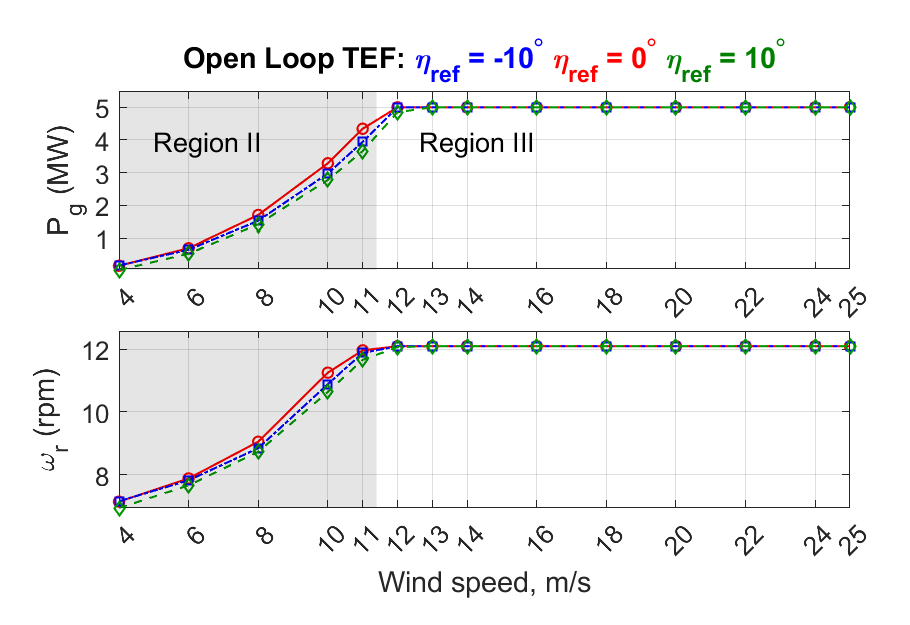
\includegraphics[width=0.485\textwidth]{figures/Images_Torque24/fig06_TEFOL_1.eps}}\hfill 
\subfloat[Rotor thrust and blade pitch]{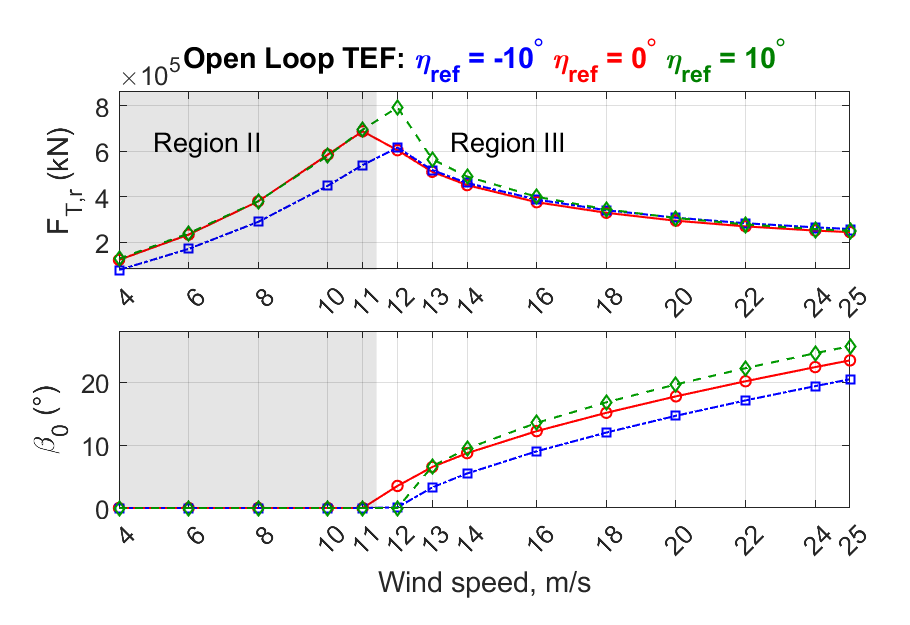
\includegraphics[width=0.485\textwidth]{figures/Images_Torque24/fig06_TEFOL_2.eps}}\hfill
%\subfloat[blc blc]{\includegraphics[width=0.31\textwidth]{figures/twoTurbinesGreedyOpt_2d.eps}}
\caption{TEF open-loop verification, TEF deflection at -10\textdegree{}\,(blue), 0\textdegree{}\,(red), and 10\textdegree{}\,(green).}
\label{fig:OLval}
\end{figure}

%
The simulated power with and without TEF deflections shows the expected power characteristic curve of a wind turbine: In Region~II, both positive and negative flap deflections reduce power \(P_g\) due to decreased aerodynamic efficiency, unlike in Region~III, where the same power output is observed, as the power controller controls the pitch angle once rated wind speed is reached. Adjusting the pitch changes the aerodynamic forces. The control system can therefore maintain nominal power. This also reflects on the rotor speed \(\omega_r\), depicted in the second plot, which is slightly lower in Region~II but unchanged in Region~III. The thrust \(T_r\) in Region~II is decreased by a negative flap angle, while the influence of a positive flap angle on the thrust is negligible: The thrust cannot be increased beyond the neutral flap position due to the limited wind power, which necessarily limits the amount of energy converted into rotational energy. This leads to a dynamic equilibrium where, despite positive flap deflection, the thrust forces remain at levels equivalent to those at the neutral flap position. The second plot in Figure~\ref{fig:OLval}\,(b) shows the blade pitch \(\beta_{0}\), which is lower for a negative and higher for a positive TEF angle, corresponding to the lower and higher thrust force.

Figure~\ref{fig:PSDTEF} shows the power spectral density (PSD) of the blade root bending moment in closed-loop for the first verification data set with a mean wind speed of 16 m/s. 
\begin{figure} [h]
    \subfloat[Baseline (black), IPC (blue), and IFC (green)]{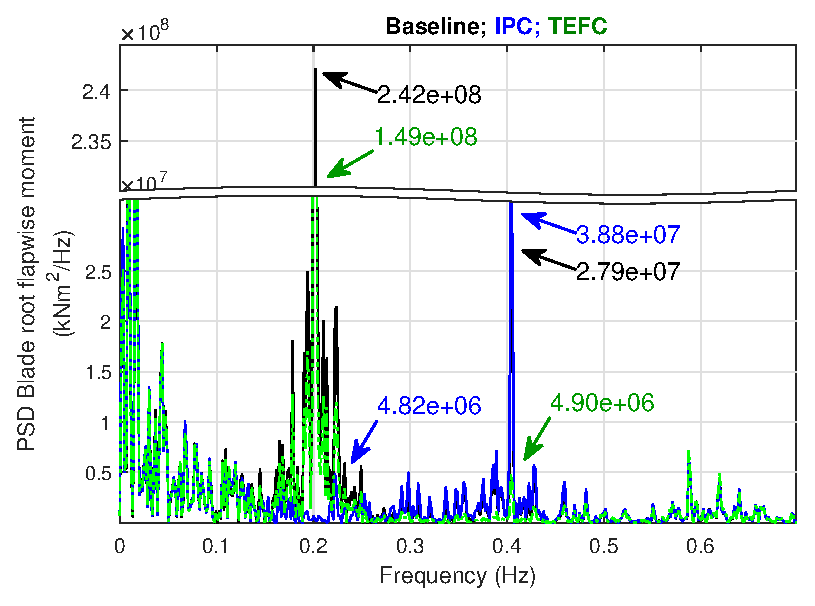
\includegraphics[width=0.485\textwidth]{figures/Images_Torque24/fig02_PSDroot_breaky.eps}}\hfill 
    \subfloat[AALC (red), and AALC optimized (pink)]{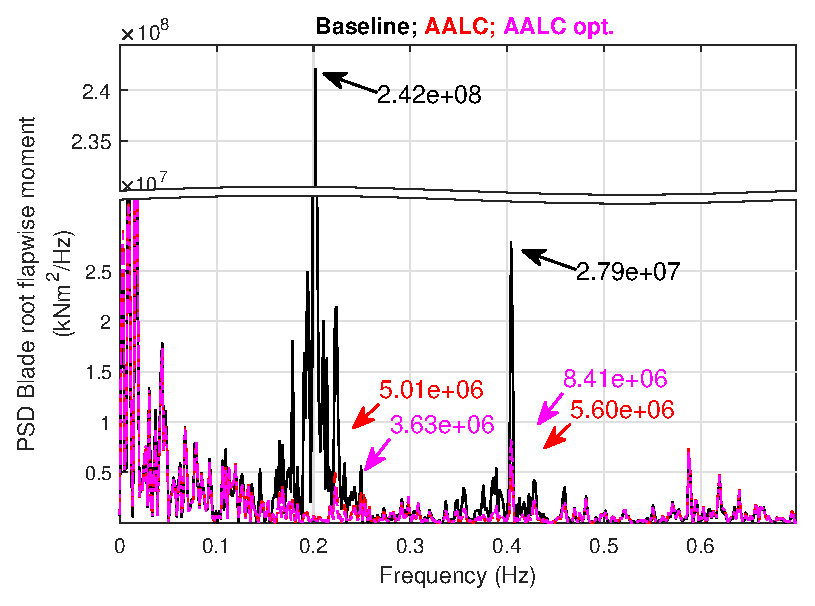
\includegraphics[width=0.485\textwidth]{figures/Images_Torque24/fig02_PSDroot_breaky1c.eps}}\hfill
    %\subfloat[blc blc]{\includegraphics[width=0.31\textwidth]{figures/twoTurbinesGreedyOpt_2d.eps}}
    \caption{Power Spectral Density of optimization set signals, turbulence class A, with mean wind speed 16~m/s.}
    \label{fig:PSDTEF}
\end{figure}
%    
IPC (blue line) and IFC (green line) reduce the PSD of the 1P and 2P loads, respectively, compared to the baseline (black line). These PSDs are obtained with the initially used AALC parameters with the original setting of a purely integral IPC and a purely proportional IFC feedback, both set to values of one. In a first optimization step, only the two controller parameters \(K_{I,\text{IPC}}\) and \(K_{P,\text{IFC}}\) are optimized. In a second step, the four additional parameters of the two PI controllers are optimized as well, resulting in an IPC PI controller, with $K_{P,\text{IPC}} = 0.354$ and $K_{I,\text{IPC}}= 1.194$ and an IFC P controller with $K_{P,\text{IPC}}= 0.631$. 

Figure~\ref{fig:PSDTEF}\,(b) demonstrates that considerable improvement with respect to the baseline controller is possible using the suggested AALC design: The combined IPC-TEFC with the original setting of a purely integral IPC and proportional TEFC feedback reduces the PSD at 1P by 97.9\%, and at 2P by 79.9\%. Adding and optimizing additional parameters improves the AALC's effect only slightly further, with a reduction at 1P of 98.5\% and 2P of 69.8\% with respect to the baseline. With regard to the selected starting values of the AALC, this is a further reduction at 1P of 27.5\%, but an increase at 2P of 50.1\%. The cost function of the two controllers is at $J = 0.880$ for the initial controller and at $J = 0.877$ for the optimized one. This illustrates that while the optimization objective, the reduction in blade DEL, was achieved as desired, the slightly reduced effectiveness at the 2P frequency peak may lead to a slightly lower reduction in tower DEL.
From this study, it seems unlikely that a parameter optimization of the suggested, carefully designed controller can decrease the blade damage equivalent loads considerably. Further investigations might be made with respect to how much improvement is achievable with a more sophisticated MIMO controller. 

Apart from the blade root flapwise moment, the influence of the obtained controller parameters is compared with respect to the evaluation criteria provided in section \ref{sec:ControllerParameterOptimization}.
Table~\ref{tabone} contains the five evaluation criteria to quantify the effect of the AALC: Blade and tower DEL, mean of generated power $\bar{P}_{g}$, its standard deviation $\sigma P$, and actuator power $P_{\text{Act}}$. The mean of the five criteria for all five simulations covering the part of Region~III above 16\,m/s is normalized through simulations without AALC with the same wind test cases. Blade DEL decrease by 20\% and 22\%.  Tower bottom DEL and top DEL are decreased by between 1\% and 3\% for the verification sets.
\begin{table}[h]
    \centering
    \caption[Wind turbine evaluation criteria for IPC-TEFC: Mean values optimization and verification data sets]{\label{tabone} Wind turbine evaluation criteria for AALC: Mean values optimization and verification data sets averaged over the values of wind test cases from 16\,m/s to 25\,m/s. Criteria are tower base, tower top and blade DELS, and power mean and standard deviation.}
    \begin{tabular}{@{}*{8}{c}@{}}
       Data set & Turb. class & $C_{\text{DEL},b}$ & $C_{\text{DEL},t,\text{Base}}$ & $C_{\text{DEL},t,\text{Top}}$ & $C_{\bar{P}}$ & $C_{\delta P}$ & $C_{\text{Act}}$ \\
        \hline
        Optim.   & A & 0.77 & 0.98 & 0.96 & 1.00 & 1.00 & 3.94 \\
        Verif. 1 & A & 0.80 & 0.99 & 0.98 & 1.00 & 1.01 & 3.84 \\
        Verif. 2 & B & 0.78 & 0.99 & 0.97 & 1.00 & 1.01 & 4.09 \\
    \end{tabular}
\end{table}

 The evaluation of the power criteria confirms that the AALC leads only to negligible changes in both power mean and variance. The additional rotational movement of the blade demanded by IPC is the only criterion leading to an unavoidable increase, similar to the two controller schemes discussed in previous sections. To assess the overall performance of AALC relative to the other discussed control strategies, the following section presents a comparison of all three investigated algorithms on load reduction and  power standard deviation at different pitch rate limits. 

\subsection{Comparison of Wind Turbine Control Designs}
\label{subsec:ComparisonWindTurbineControlDesigns}

Figure~\ref{fig:CtrlCompAll} shows the evaluation criteria for blade DEL $C_\text{DEL,b}$,
tower DEL $C_\text{DEL,t}$, and power standard deviation $C_{\delta P}$ as a function
of actuator activity criterion $C_\text{Act}$ for qLMPC, IPC, and AALC, evaluated for normal
turbulent wind of turbulence class~B and a mean wind speed of 16\,m/s from the second verification test set. All criteria are normalized by the corresponding values of the PI CPC baseline, so that values below unity
indicate improvement. 
  \begin{figure}[h]
     \begin{center}
         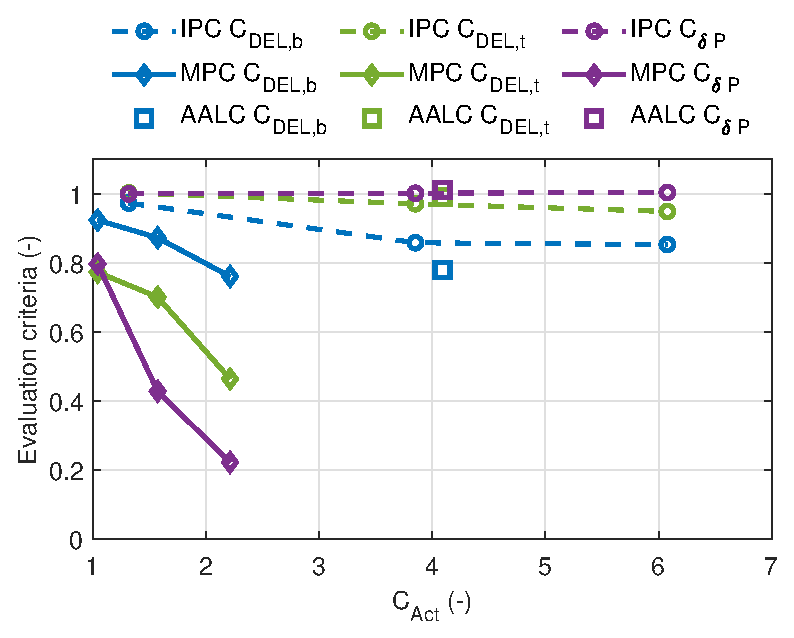
\includegraphics[width=0.65\textwidth]{figures/figures_WESC25/afig01_IPCMPCpareto.eps}
         
 
\caption[Evaluation criteria for qLMPC, IPC, and AALC for turbulent wind.] { Evaluation criteria for qLMPC, IPC, and AALC for turbulent wind (16\,m/s mean, IEC turbulence class B (14\%)). Criteria are tower base and blade DELs, power mean and standard deviation, and actuator power.}
         \label{fig:CtrlCompAll}
     \end{center}
 \end{figure}
 For qLMPC and IPC, three pitch rate limits were tested, resulting
 in different points along the actuator activity axis. Dashed lines with circles as markers show the result of IPC and solid lines with diamond markers the one obtained with qLMPC. The AALC optimization was run with a fixed pitch rate limit of 8\textdegree/s. Hence, only a single point, marked with a square, exists for AALC for each of the three criteria. As before, the blade and tower DEL lines are depicted in blue and green, respectively, and the power standard deviation in purple. The points with the smallest actuator criterion correspond to the numbers obtained with the rate limit of 4\textdegree/s and the ones with the largest to the values calculated for the rate limit of 13\textdegree/s.
 An important distinction between the three approaches is their effect on power variability.
 IPC and AALC only change $C_{\delta P}$ negligibly, with results at or marginally above unity, indicating that they
 preserve or very slightly increase power variance relative to the PI baseline. In contrast,
 qLMPC is the only controller that actively reduces power variance, with $C_{\delta P}$
 dropping to approximately 0.22 at the highest pitch rate limit. This is a direct consequence
 of the MIMO formulation of qLMPC, which simultaneously optimizes pitch and torque to
 minimize both structural loads and power fluctuations, whereas IPC and AALC operate as
 SISO pitch controllers without an explicit power smoothing objective.  The steep shape of the Pareto front $C_{\delta P}$ for qLMPC reflects that changes in the rotor and generator speed are penalized in the cost function. In Region III, where the turbine is operated around the rated generator torque and rated power, changes in power depend linearly on generator speed changes. As these are reduced considerably with the proposed qLMPC scheme, a smoother power yield is achieved.
 
 
 Tower DEL reductions, by contrast, are a byproduct of the more aggressive pitch actuation smoothing the aerodynamic thrust. The resulting fluctuations are the main source of tower fore-aft excitation and, to a lesser degree, of blade loads. As they are not directly included in the MPC cost function, their lines are flatter and do not show the curvature of a typical Pareto front.
 
All three controllers reduce blade and tower DELs relative to
 the PI baseline while maintaining the same mean power output. qLMPC consistently
 outperforms IPC across all three pitch rate settings, achieving lower DELs at comparable
 actuator activity. The AALC result at $C_\text{Act} \approx 4.2$ suggests that combining
 IPC with trailing edge flaps achieves blade DEL reductions comparable to qLMPC at lower
 pitch actuator demand, indicating that TEFs may offer a promising path to further blade
 load reduction without increasing pitch activity by an unacceptable factor.
 
 These results must be interpreted with caution, as the turbine and prediction models used
 in qLMPC are currently identical, which is unlikely to reflect real deployment conditions.
 Nevertheless, considerable improvements over baseline PI control are still expected, as
 reported in other MPC applications. The reliance of qLMPC on accurate wind preview
 information also presents a practical challenge.
 
 IPC, while delivering the least improvement of the three approaches, achieves reductions
 in the two-digit percentage range without requiring wind measurements or additional
 actuation hardware. AALC outperforms IPC by offloading part of the pitch actuation effort
 onto the trailing edge flaps, resulting in greater DEL reductions at lower pitch activity.
 These results highlight the trade-offs between controller complexity, sensor requirements,
 additional hardware such as TEFs, and load mitigation performance. The presented qLMPC offers
 the greatest potential for multi-objective control and is the only approach
 among the three that reduces power variability, but IPC remains a practical
 solution when lidar wind preview data is unavailable. 
 
 The presented qLMPC exploits that individual wind turbine dynamics are well understood and can be described in closed
 form as low-dimensional nonlinear ODEs. The following chapter discusses data-driven MPC for wind farms,
 where wake dynamics are time- and location-dependent and cannot be described by
 closed-form ODEs, yet must be accounted for in any MPC formulation.
 

 
 
 